%%%%%%%%%%%%%%%%%%%%%%%%%%%%%%%%%%%%%%%%%%%%%%%%%%%%%%%%%%%%%%%%%%%%%%%%%%%%%%%
% Fraction of gluon splitting in data
%%%%%%%%%%%%%%%%%%%%%%%%%%%%%%%%%%%%%%%%%%%%%%%%%%%%%%%%%%%%%%%%%%%%%%%%%%%%%%%
%
\chapter{Fraction of double {\em b\hspace{.5mm}}-hadron jets in QCD {\em b\hspace{.5mm}}-production}\label{ch:gbbfraction}


In this chapter we apply the newly developed $g \rightarrow b\bar{b}$ tagging tool to measure the fraction of merged $b$-jets in QCD $b$-jet production. The fractions are determined both for an inclusive $b$-jets sample with $|\eta|<2.1$, and for exclusive samples enriched in single or in merged $b$-jet.
The measured fractions are in excellent agreement, within the experimental uncertainties, with the theoretical predictions from a simulation of hadronic collisions.
%The chapter is organized as follows. Section~\ref{sec:FitIntro} introduces the concept of template fitting. Section~\ref{sec:LLFits} describes the statistical method used to perform the template fits.


%------------------------------------------------------------------------
\section{Introduction}\label{sec:FitIntro}
%------------------------------------------------------------------------

The $g\rightarrow b\bar{b}$ tagger developed and described in the previous chapters produces for every $b$-tagged jet a number between 0 and 1, the double $b$-hadron likelihood (LL). The closer this number is to 1 (0), the more likely the $b$-tagged jet is single (merged). When used as a tagger, a working point (Wp) is chosen so that if LL$\geq$Wp the jet is flagged as single. The value of Wp is chosen as a compromise between good efficiency (the lower the Wp, the lower the probability that an actual single $b$-jet will be missed by the tagger), and rejection power (the higher the Wp the lower the probability that a non-single $b$-jet will be incorrectly flagged as single). Depending on the necessities of the particular analysis, an appropriate Wp is to be chosen from the plot in Figure~\ref{fig:performanceinbins}. In particular, the performance results presented in Chapter~\ref{ch:mva} correspond to the 50\% and 60\% efficiency working points, two reasonable choices.

However, the values of LL in a given sample offer more information than just a jet-by-jet tagger: the distribution of LL allows to measure the composition of the particular sample. In effect, a $b$-tagged jet has a certain probability to actually originate from the hadronization of:

\begin{itemize}
\item
$b$: a $b$-quark
\item
$b\bar{b}$: gluon splitting into a $b\bar{b}$ pair
\item
$c$: a $c$-quark
\item
$c\bar{c}$: gluon splitting into a $c\bar{c}$ pair
\item
$\ell$: a light parton ($u$, $d$, $s$ quarks, or a $g$ not splitting into heavy flavor)
\end{itemize}

The expected distribution of LL is different for each of the five cases. This is illustrated in Figure~\ref{fig:templates}, which plots LL for each hypothesis for jets in a $\pt$ range representative of the energy covered in the analysis ($80<\pt\leq110$~GeV). These distributions are henceforth called ``templates''. 
\begin{figure}[htb]
\centering
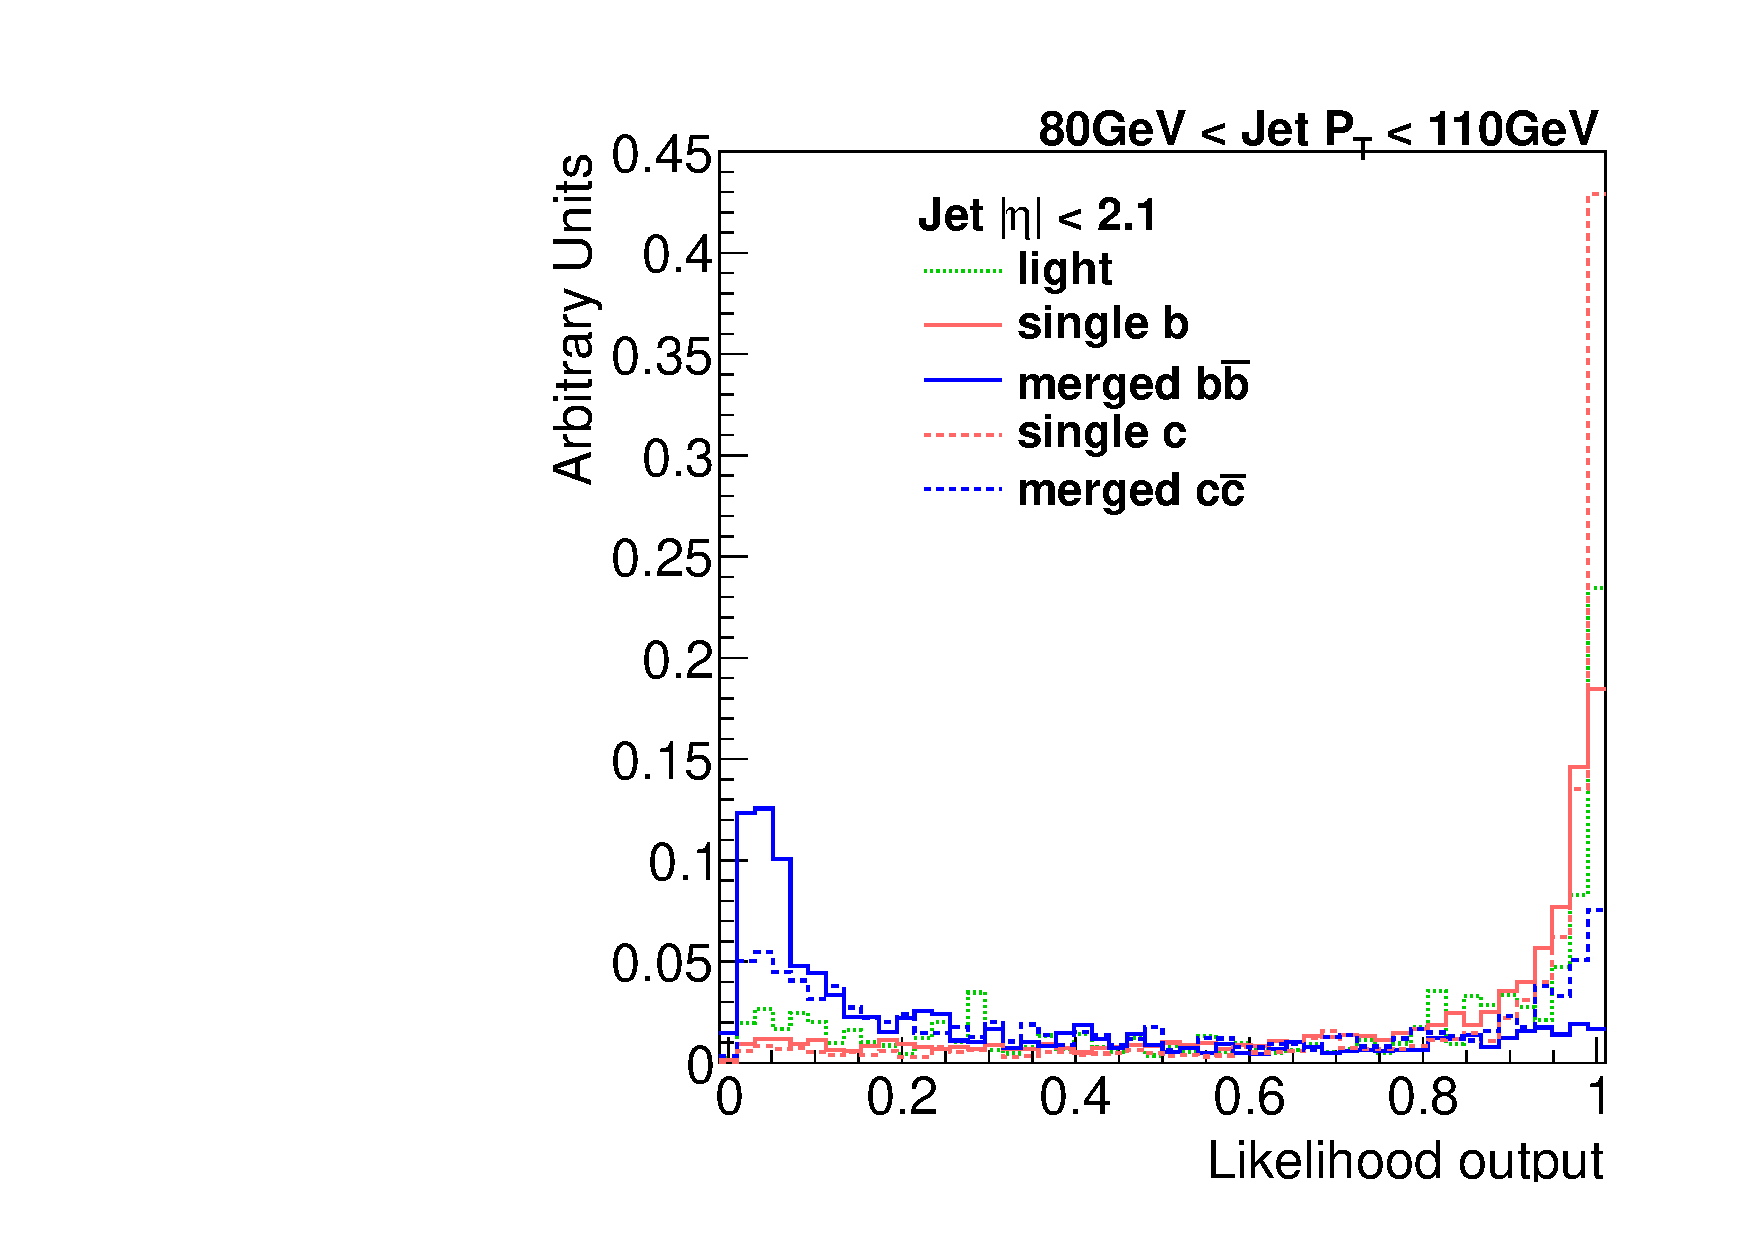
\includegraphics[width=0.80\textwidth]{FIGS/Fits/AllTemplates080.pdf}
%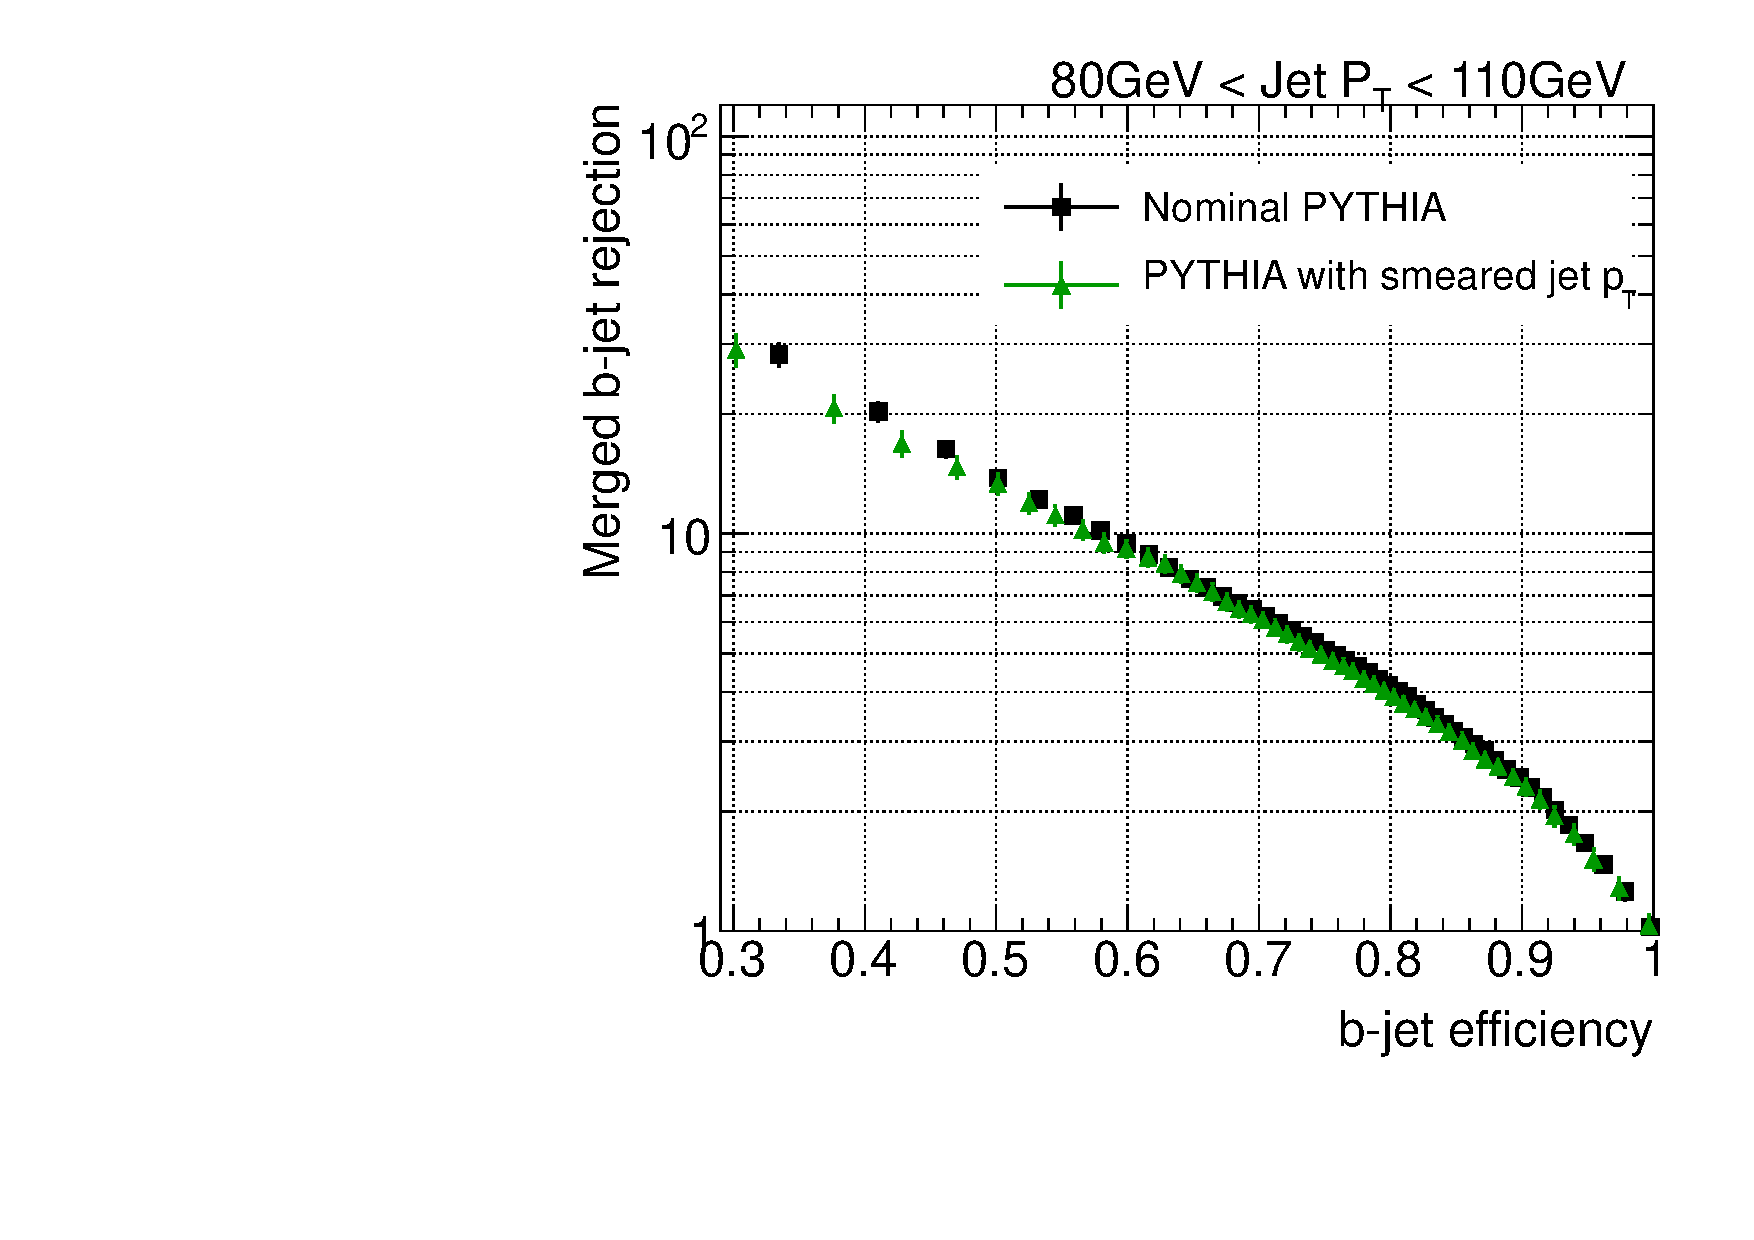
\includegraphics[width=0.49\textwidth]{FIGS/systematics/LlhoodKDE_ISO_SmearedJetPt_FIXEDBUGTest_rejvseff080.pdf}
\caption{Likelihood distribution for the five flavours, $b$, $c$, $b\bar{b}$, $c\bar{c}$ and $\ell$ are shown for $b$-tagged jets in the simulated QCD sample. The templates are all normalized to unit area to allow the comparison.}
\label{fig:templates}
\end{figure}
The shape of the distributions in Figure~\ref{fig:templates} can be intuitively understood. The $b$ and $b\bar{b}$ templates behave as expected, respectively peaking at high and low values of LL. The $c$ template resembles its $b$ counterpart. The $c\bar{c}$ although similar to the $b\bar{b}$ template, also exhibits a spike for large values of LL.  
%This was to be expected, given that a $c$-quark fragments mainly into into $D$-mesons which have a measurable $c\tau$ of $\sim$300$\mu$m shorter than the  $c\tau$ of $\sim$500$\mu$m corresponding to the $B$-mesons produced in $b$-quark fragmentation. 
This was to be expected, given that $c$-jets have less tracks than $b$-jets: they decay to $D$ mesons, $c \rightarrow D \rightarrow \mbox{light hadrons}$, as opposed to $b$-jets which present a longer decay chain, $b \rightarrow B \rightarrow D\rightarrow \mbox{light hadrons}$. They also show smaller angular separation (width), since $m_D < m_B$  ($m_D\sim 1.9$~GeV and $m_B \sim 5.3$~GeV).
Single and merged $c$-jets are thus the main background to $b$- and $b\bar{b}$-jets. The template of light jets  %on the contrary, do not contain large decay-length secondary vertices,and its distribution is driven by...}
is comparable to the distributions observed in single $b$/$c$ jets. This can be traced to observation that gluons and light-quarks jets tend to be narrower and have lower track multiplicity than heavy-flavour jets, leading to a more single-like likelihood distributions (see Section~\ref{sec:gbbKine}).


One can determine the composition of a given sample by measuring the values of LL of the $b$-tagged jets and estimating the fractions needed from each of the templates to accurately describe the experimental LL distribution. This process is known as ``template fitting'', see Section~\ref{sec:FitsResults}. The measured composition can then be compared to the theoretical prediction from QCD. 
\begin{figure}[htb]
\centering
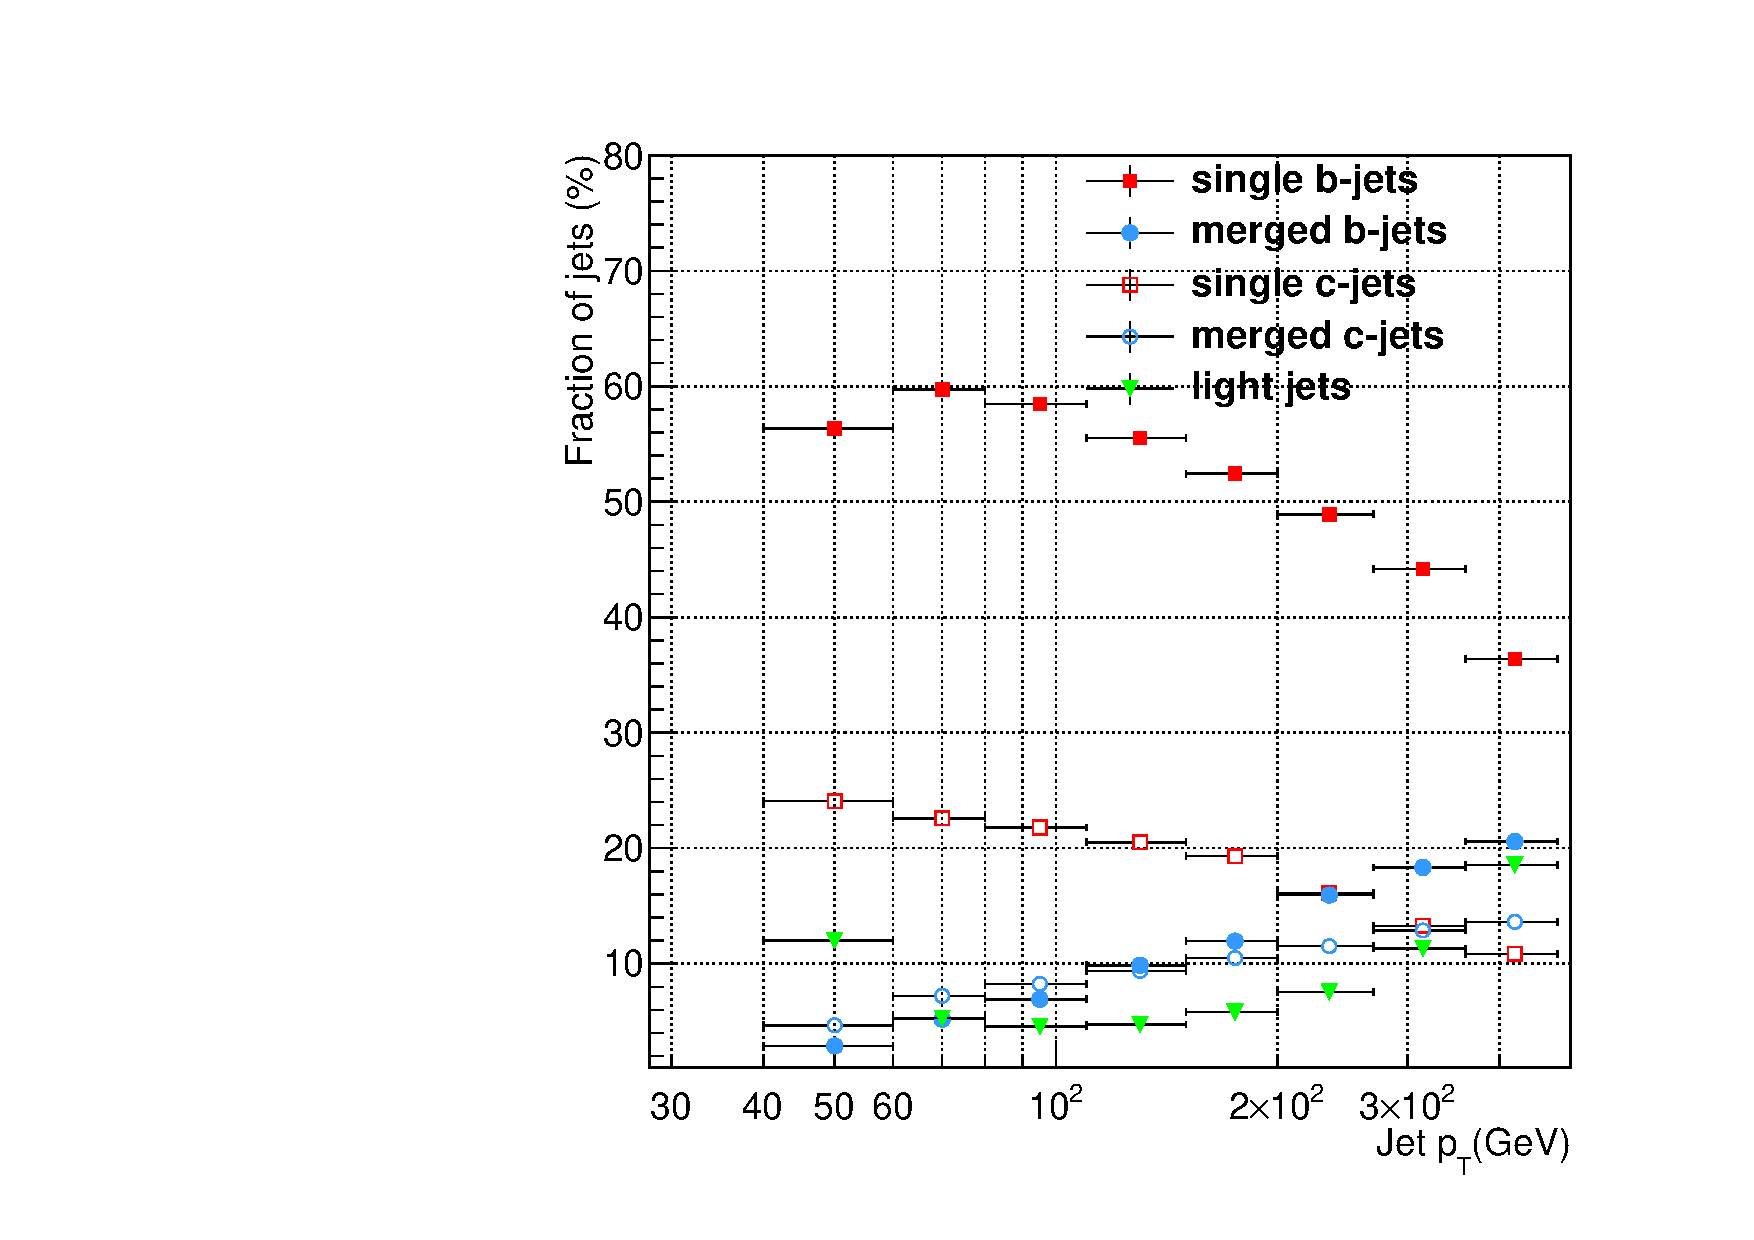
\includegraphics[width=0.70\textwidth]{TrueFractions_NominalPythia.pdf}
%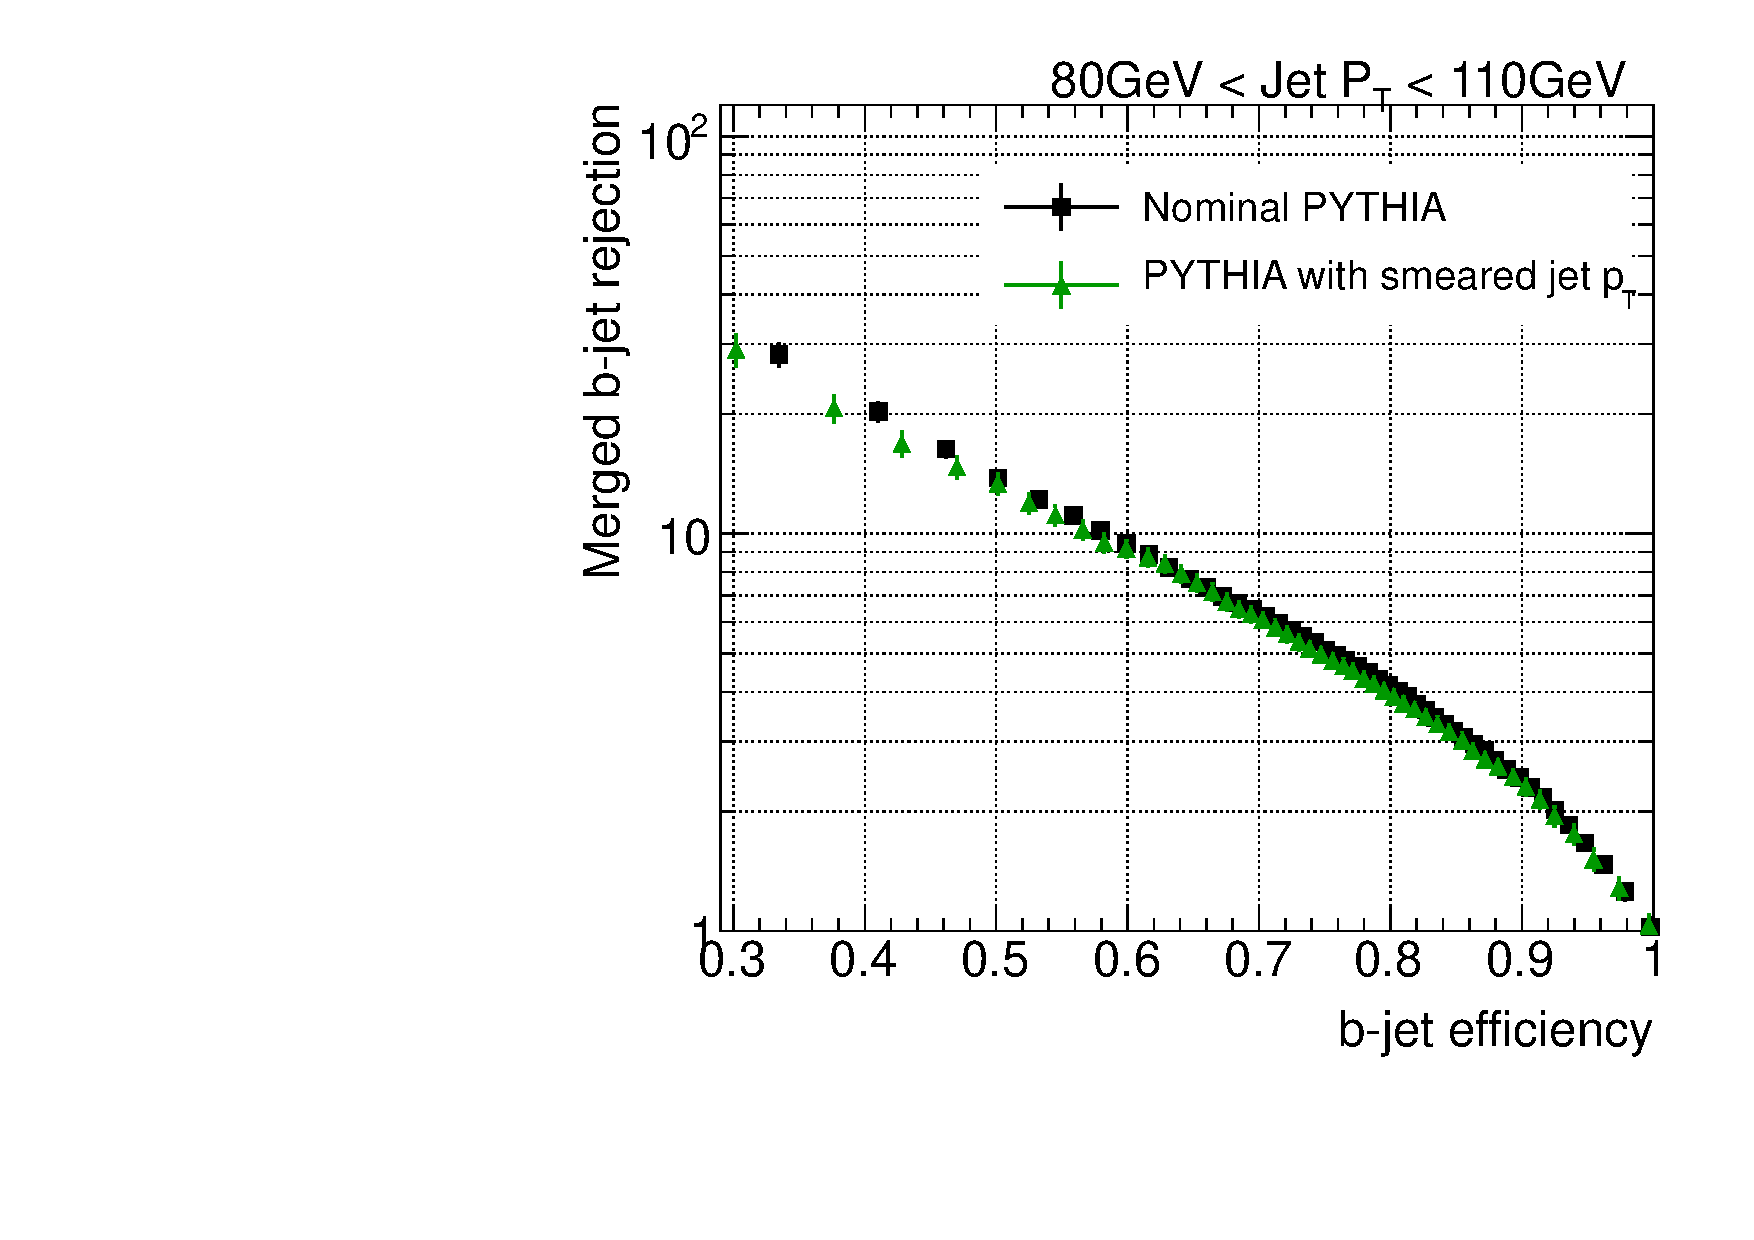
\includegraphics[width=0.49\textwidth]{FIGS/systematics/LlhoodKDE_ISO_SmearedJetPt_FIXEDBUGTest_rejvseff080.pdf}
\caption{Theoretical predictions of the fractions of $b$-, $b\bar{b}$-, $c$-, $c\bar{c}$-, and $\ell$-jets in $b$-tagged jets from a {\sc Pythia} simulation of QCD jet production.}
\label{fig:truefractions}
\end{figure}
Figure~\ref{fig:truefractions} shows the expected fractions as a function of $\pt$ from a {\sc Pythia} simulation of QCD jet production in $pp$ collisions at 7~TeV. We observe that the fraction of single (merged) $b$-jets tends to decrease (increase) with $\pt$. This is expected as, with increasing $\pt$, the larger the boost of the $b\bar{b}$ pair produced by gluon splitting, and the higher the probability that they will be produced at a small angle and reconstructed within the same jet. The fraction of merged jets is slightly smaller for the first $\pt$ bin because the $b$-tagging efficiency drops at low $\pt$, bringing about a larger fraction of light jets. 


%------------------------------------------------------------------------
\section{Unbinned maximum likelihood fits}\label{sec:LLFits}
%------------------------------------------------------------------------

The analysis of experimental data often involves the estimation of the composition of a sample, based on Monte Carlo description of the various sources. We measure a number of observables $x_i$ and we want to determine one or more parameters $p_i$ from the data, such as the number of signal and background events. The distribution  of the observables is described by a probability density function (PDF), which is a function of %both the observables and 
the parameters, $F(\vec{x},\vec{p})$.  We choose the PDF based on some hypothesis about what function would match the data, and vary the parameters in order to make the PDF match the distribution of the observables as well as possible. 


In the case of data binned into a histogram, one approach is to use a least-squares fitting technique to estimate the parameters. They are adjusted to minimize
%
\begin{equation}
\chi^2 = \sum^n_i \frac{(d_i - f_i)^2}{d_i}
 \label{eq:chi2}
\end{equation}
%
where $d_i$ is the number of data events that fall into bin $i$; $n$ is the number of bins, and $f_i$ is the predicted number of events in bin $i$, defined by
%
\begin{equation}
f_i = N_D\sum^m_{j=1} p_j \cdot a_{ji}/N_j
\end{equation}
%
with $p_j$, the proportions of the different $m$ sources; $a_{ij}$, the number of Monte Carlo events from source $j$ in bin $i$, with $i=1,2,...,n$; $N_D$, the total number of events in the data sample; and $N_j$, the total number in the MC sample for source $j$.

This $\chi^2$ assumes that the distribution for $d_i$ is Gaussian and that $a_{ij}$ has no uncertainty. The distribution of $d_i$ is of course Poisson, but the Gaussian $N(\mu = d_i,\sigma = \sqrt{d_i})$ is a good approximation for large  $d_i$.  Unfortunately it often happens that many of the $d_i$ are small, making the $\chi^2$ value given in Equation~\ref{eq:chi2} inappropiate to describe the problem.  Instead one can go back to the original Poisson distribution, and write down the probability for observing a particular $d_i$ as
%
\begin{equation}
e^{-f_i} \frac{f_i^{d_i}}{d_i!} 
\end{equation}
%
and the estimates of the proportions $p_j$ are found by maximizing the total likelihood, 
%
\begin{equation}
\mathcal{L} = \prod^n_{i=1} e^{-f_i} \frac{f_i^{d_i}}{d_i!}.
\end{equation}
%
This accounts correctly for bins with small numbers of events.  It is often referred to as a ``binned maximum likelihood'' fit. Actually this formalism does not account for fluctuations in the $a_{ji}$ due to finite Monte Carlo samples. A similar methodology that correctly describes this scenario exists, see Ref.~\cite{Barlow1993219}. The effects of finite MC data size can be considered small for MC samples ten times larger than the data sample. 


The technique of binned maximum likelihood fit is fast and analytical; %unfortunately, 
however, we observed that the obtained uncertainties were unnaturally large.  This was traced to the use of events with rather different weights. In effect, Ref.~\cite{Barlow1993219} reports that this method only works satisfactory with weighted events if the weights do not differ very much~\cite{Barlow1993219}.
We had thus to move to a different, more general technique, an ``unbinned maximum likelihood fit'',  which allows arbitrary weights and has the further advantage of using all the information contained in the data sample; although it is not analytical but numerical and iterative. 
%The binned maximum likelihood fits is a technique in general use. Unfortunately  this method does not behave well in problems where it is necessary to apply weights to the Monte Carlo, such as in our composite dijet sample. We will use instead a different technique for fitting, an ``unbinned maximum likelihood fit'', which does support weighted datasets. %But use with care. Error analysis in ML fits to weighted unbinned data can be complicated...
%Binned or unbinned MF fit. %Roofit presentation page 112
%In most RooFit applications it doesn't matter. Internally binned data is represented the same way as unbinned data, a ROOT TTree with the bin coordinates.

The likelihood to be maximized in an unbinned dataset of events $\{\vec{x}_k\}^N_{k=1}$ is the product of the $F(\vec{x},\vec{p})$ PDF over all events
%
\begin{equation}
\mathcal{L}(\vec{x};\vec{p}) =\prod^N_{k=1} F(\vec{x}_k;\vec{p})
\end{equation}
%
which, can be rewritten in terms of distribution the probability of oberving an event from source $j$ in the sample,
%
\begin{equation}
\mathcal{L} =  \prod^N_{k=1} \sum^m_{j=1} p_j  \mathcal{T}_j(\vec{x}_k)
 \label{eq:LLgeneral}
\end{equation}
%
where $\mathcal{T}_j$ are the PDFs that represent the distribution of $\vec{x}_k$ for each of the $m$ hypothesis, $p_j$ are the parameters representing the proportions for the $j^{th}$ hypothesis, and $N$ is the total number of input data points.

%\subsubsection{Extended maximum likelihood fits}

%Maximum likelihood information only parametrizes the shape of a distribution; that is, one can determine fraction of signal events from MC fits but no number of signal events. The extended version of the maximum likelihood approach adds an extra term allowing the estimation of %the absolute number of signal/background events. 
%a parameter that represents the number of events in the sample, $N_{exp}$.
%The extra term describes the probability of observing the actual number of events, $N_{obs}$, given this parameter. This probability is described by the Poisson distribution
%%
%\begin{equation}
%P(N_{obs},N_{exp}) \sim  N_{exp}^{N_{obs}} \cdot e^{-N_{exp}},
%\end{equation}
%%
%and we refer to the likelihood including this factor as the ``extended likelihood''
%%
%\begin{equation}
%\tilde{\mathcal{L}}(\vec{x},N_{obs};\vec{p},N_{exp}) \equiv P(N_{obs},N_{exp}) \cdot \mathcal{L}(\vec{x};\vec{p})
%\end{equation}
%%
%The fit then finds the values of $n_j$, the number of events for each hypothesis $j$. 

The PDF in~\ref{eq:LLgeneral} is the sum  of multiple probability density functions. Mathematically, the sum of two probability density functions is also a normalized probability density function as long as the coeffients add up to 1 (for simplicity we take $\vec{x}_k=x_k$),
% 
\begin{equation} 
F(x_k) = p_0 \cdot \mathcal{T}_0(x_k) + p_1 \cdot \mathcal{T}_1(x_k)+...+p_{m-1}\mathcal{T}_{m-1}(x_k)+ (1-\sum^{m-1}_{i=1}p_i) \mathcal{T}_m(x_k).
\end{equation}
%
If the sum of these coefficients becomes larger than one, the remainder coefficient will be assigned a negative fraction. As long as the summed p.d.f is greater than zero everywhere, this is not ill-defined. %but may pose some problems in the interpretation
In the case of the present analysis $x_k$ represents the double $b$-hadron likelihood, LL. 

The fits were performed in this thesis by means of the RooFit Toolkit for data modelling~\cite{RooFit}. Performing a fit consists of minimizing the negative log-likelihood of a PDF calculated over the data set % (for simplicity we drop for a moment the extra term)
%
\begin{equation}
-\log \mathcal{L} (\vec{p}) = \sum_k F(\vec{x}_k;\vec{p})
\end{equation}
%
with respect to the model's parameters.  The RooFitTools package uses the MINUIT\cite{MINUIT} algorithms to find the minimum of this function and estimate the errors in each parameter.  %fitTo() method returns an interger status code which is non-zero if the fit fails to converge normally.
%In order to assess the goodness of a fit one can compare the minimum value of the negative log-likelihood function with the expected distribution of values for samples generated according to the fit model (using the Monte Carlo study methods).
%To increse the chances of proper convergence, it is important to provide reason
%able initial estimates for the parameters to be fitted.


%\subsubsection{Model}

%Most realistic data description models are sum of multiple components. Mathematically, the sum of two probability density functions is  also a normalized probability density function as  long as the coefficients add up to 1, % (or to the total number of events for an extended maximum likelihood fit),
%%
%\begin{equation}
%M(x) = f_{sig} \cdot S(x) + (1-f_{sig}) \cdot B(x),
%\end{equation}
%%
%or generically for N components:
%%
%\begin{equation}
%S(x) = c_0 \cdot F_0(x) + c_1 \cdot F_1(x)+...+c_{n-1}F_{n-1}(x)+ (1-\sum^{n-1}_{i=1}c_i) F_n(x)
%\end{equation}
%%
%If the sum of these coefficients becomes larger than one, the remainder coefficient will be assigned a negative fraction. As long as the summed p.d.f is greater than zero everywhere, this is not ill-defined. %but may pose some problems in the interpretation



%For the extended fit (for simplicity we take the example of signal and backgrond PDFs), 
%%
%\begin{equation}
%N_{sig} = f_{sig} \cdot N_{exp}
%\end{equation}
%%
%\begin{equation}
%N_{bkg} = (1-f_{sig}) \cdot N_{exp}
%\end{equation}
%%
%so that the extended ML procedure estimates the number of singal and background events rather than a signal fraction and a total number of events.
%The uncertainties in the yields reported by the fit will include the statistical (      )                  N                    uncertainty.

%Estimated Distance to Minimum should be small O(10-6)



%------------------------------------------------------------------------
%\section{Templates to data}\label{sec:FitsResults}
\section{Measurement for the inclusive QCD sample}\label{sec:FitsResults}
%------------------------------------------------------------------------



Likelihood Monte Carlo templates were derived from the simulated QCD samples described in Section~\ref{sec:analysis}, using all jets passing the selection criteria defined in Section~\ref{sec:EventSelection}. Likelihood templates were constructed for $b$, $c$, $b\bar{b}$, $c\bar{c}$ and $\ell$ jets separately, and these were fitted to the likelihood distribution in data in order to respectively obtain the fractions of single $b$, merged $b$, single $c$, merged $c$ and light jets in the QCD sample. Merged $c$-jets (single $c$-jets) are defined as those matching exactly two (only one) $D$ hadrons, the products of the fragmentation of $c$-quarks. A jet is classified as light when it has no $B$ nor $D$ hadrons within a cone of 0.4 around its axis.

The likelihood template fits are performed using the unbinned maximum likelihood technique (see Section~\ref{sec:LLFits}) separately for each $\pt$ bin. The functional form used is
%
\begin{equation}
F(x) = p_s \cdot S(x) + p_m \cdot M(x) + p_\ell \cdot L(x) + p_{sc} \cdot S_c(x) + p_{mc} \cdot M_c(x)
\end{equation}
%
with $S(x)$, $M(x)$, $L(x)$, $S_c(x)$ and $M_c(x)$ corresponding to the template distributions for the different hypothesis; and $p_s$, $p_m$, $p_\ell$, $p_{sc}$ and $p_{mc}$ the parameters representing the respective fractions of expected events. 

The fit to the full sample of 4.7 fb$^{-1}$ of $pp$ collision data at $\sqrt{s}=7$~TeV collected by the ATLAS experiment during 2011 is displayed in Figures~\ref{fig:fittemplates1} and~\ref{fig:fittemplates2} for two representative $\pt$ bins. The vertical scale is enlarged in the lower panels to better appreciate all contributions. It can be observed that the quality of the fit is excellent.
\begin{figure}[tp]
\centering
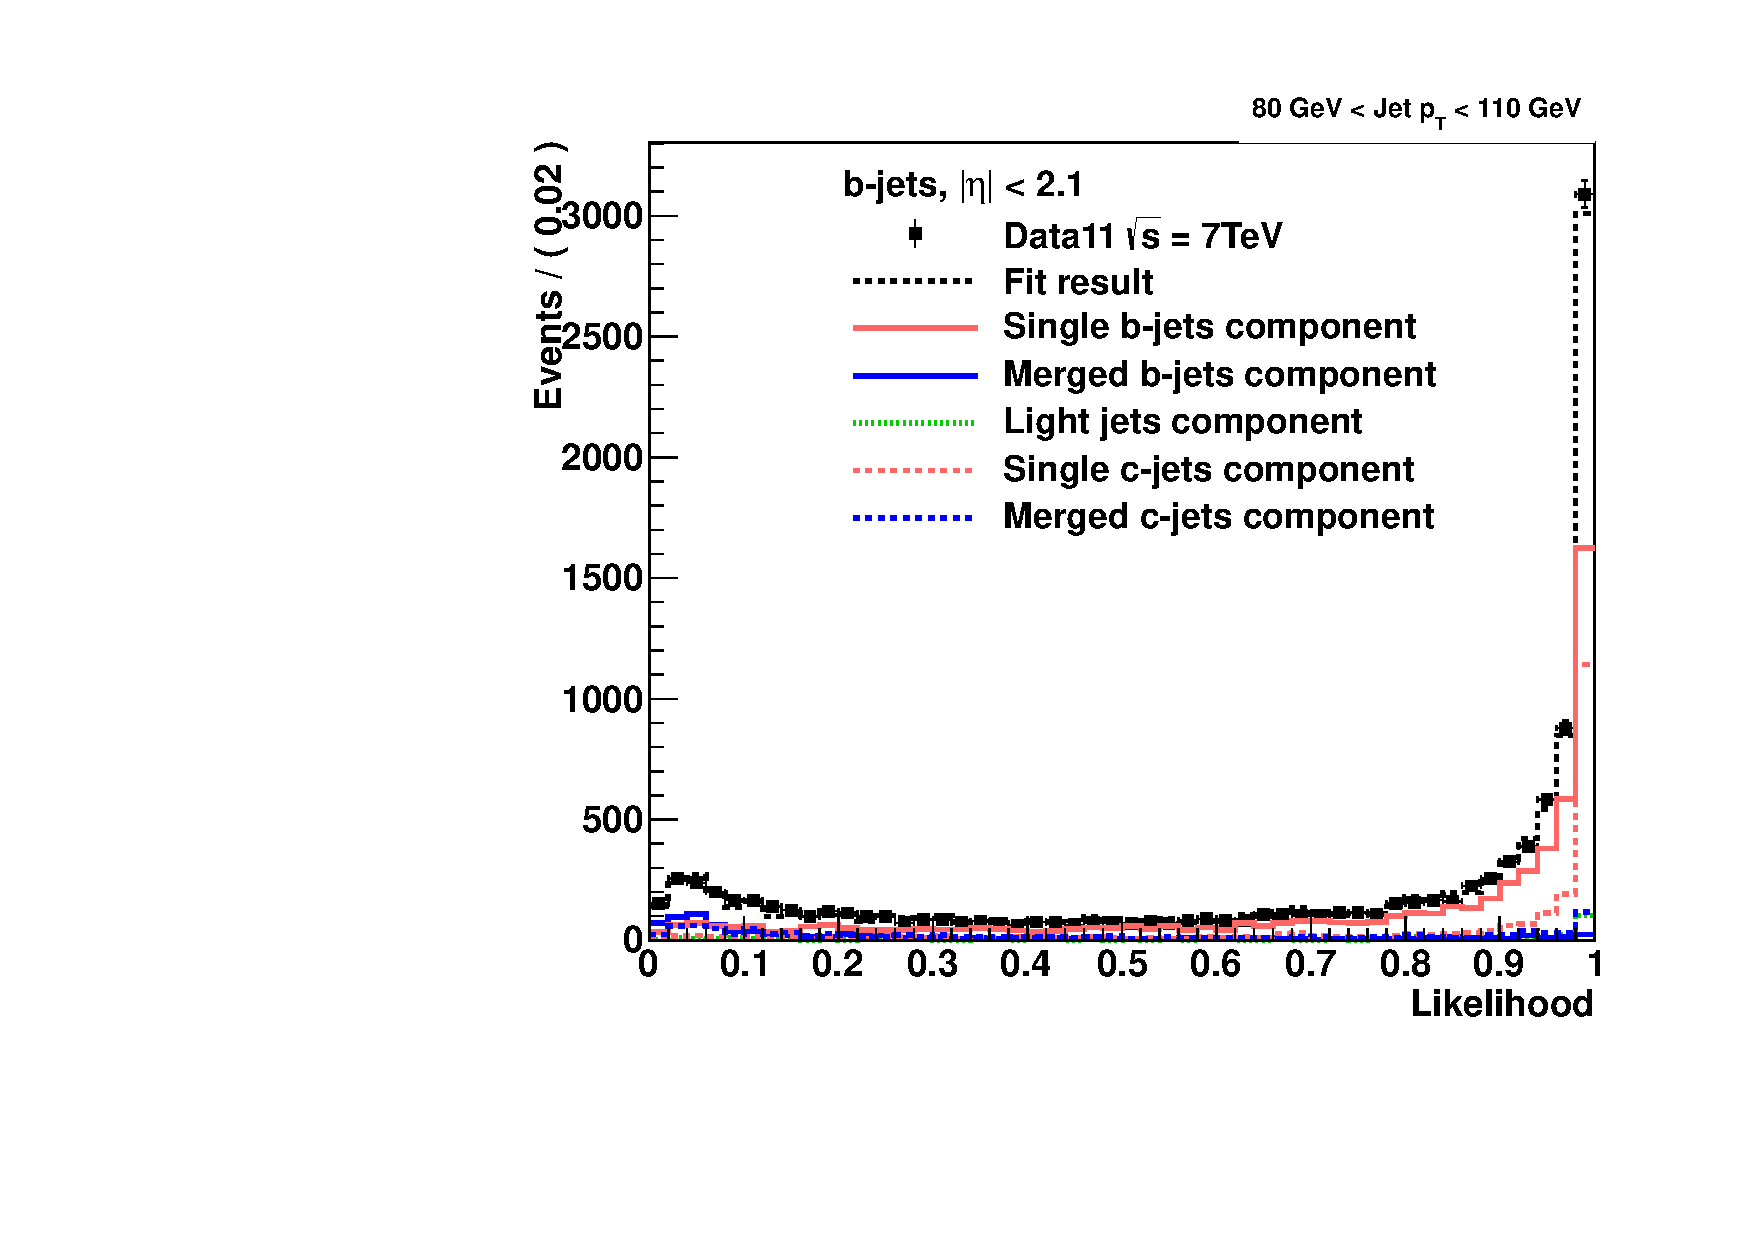
\includegraphics[width=0.7\textwidth]{FIGS/Fits/LikelihoodFit_3param_ETAFull_Bin2.pdf}
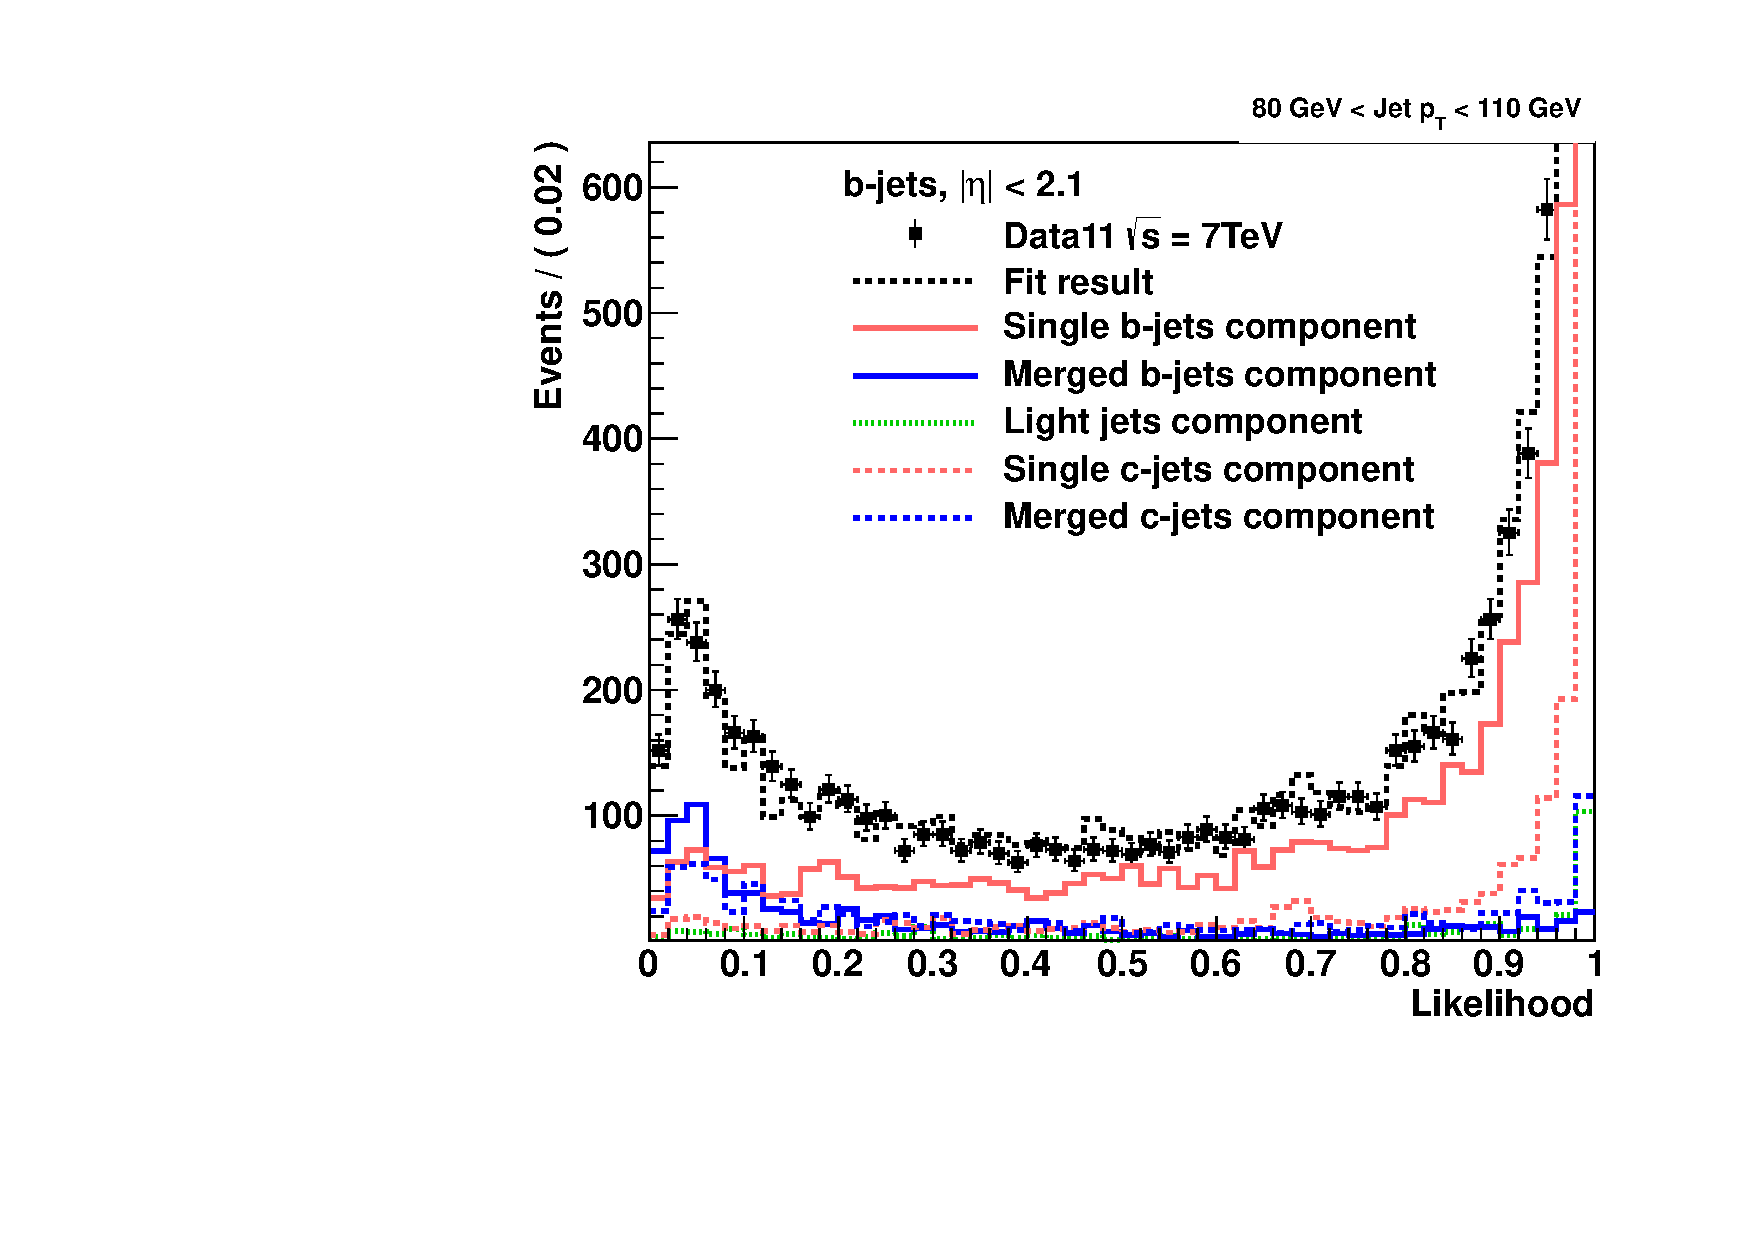
\includegraphics[width=0.7\textwidth]{FIGS/Fits/LikelihoodFit_3param_ETAFull_ZOOM_Bin2.pdf}
\caption{Example result of template fit to the likelihood distribution in data. The fit is shown for jets with $\pt$ between  80~GeV and 110~GeV, in full scale (top) and zooming the vertical scale, to better display the flavour content of the data (bottom). Uncertainties shown are statistical only.}
\label{fig:fittemplates1}
\end{figure}
\begin{figure}[tp]
\centering
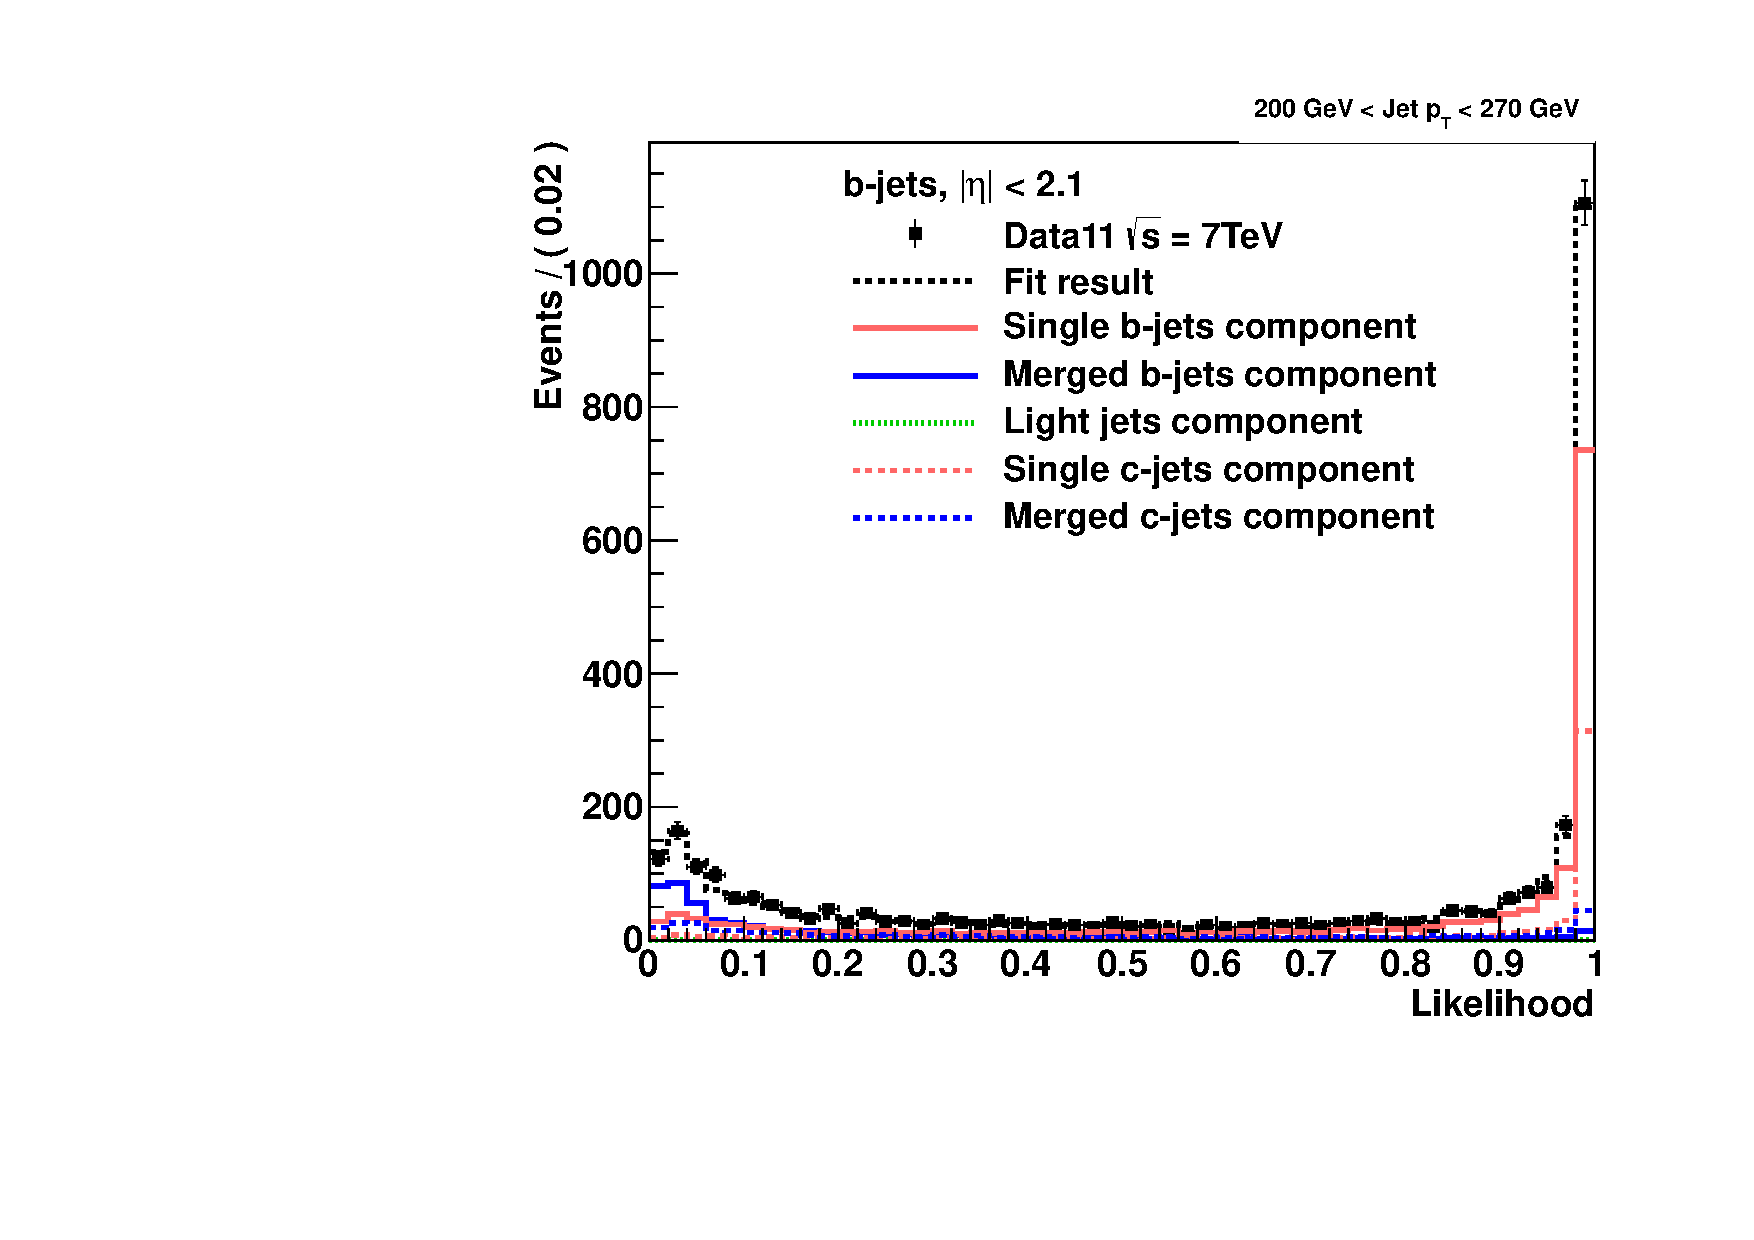
\includegraphics[width=0.7\textwidth]{FIGS/Fits/LikelihoodFit_3param_ETAFull_Bin5.pdf}
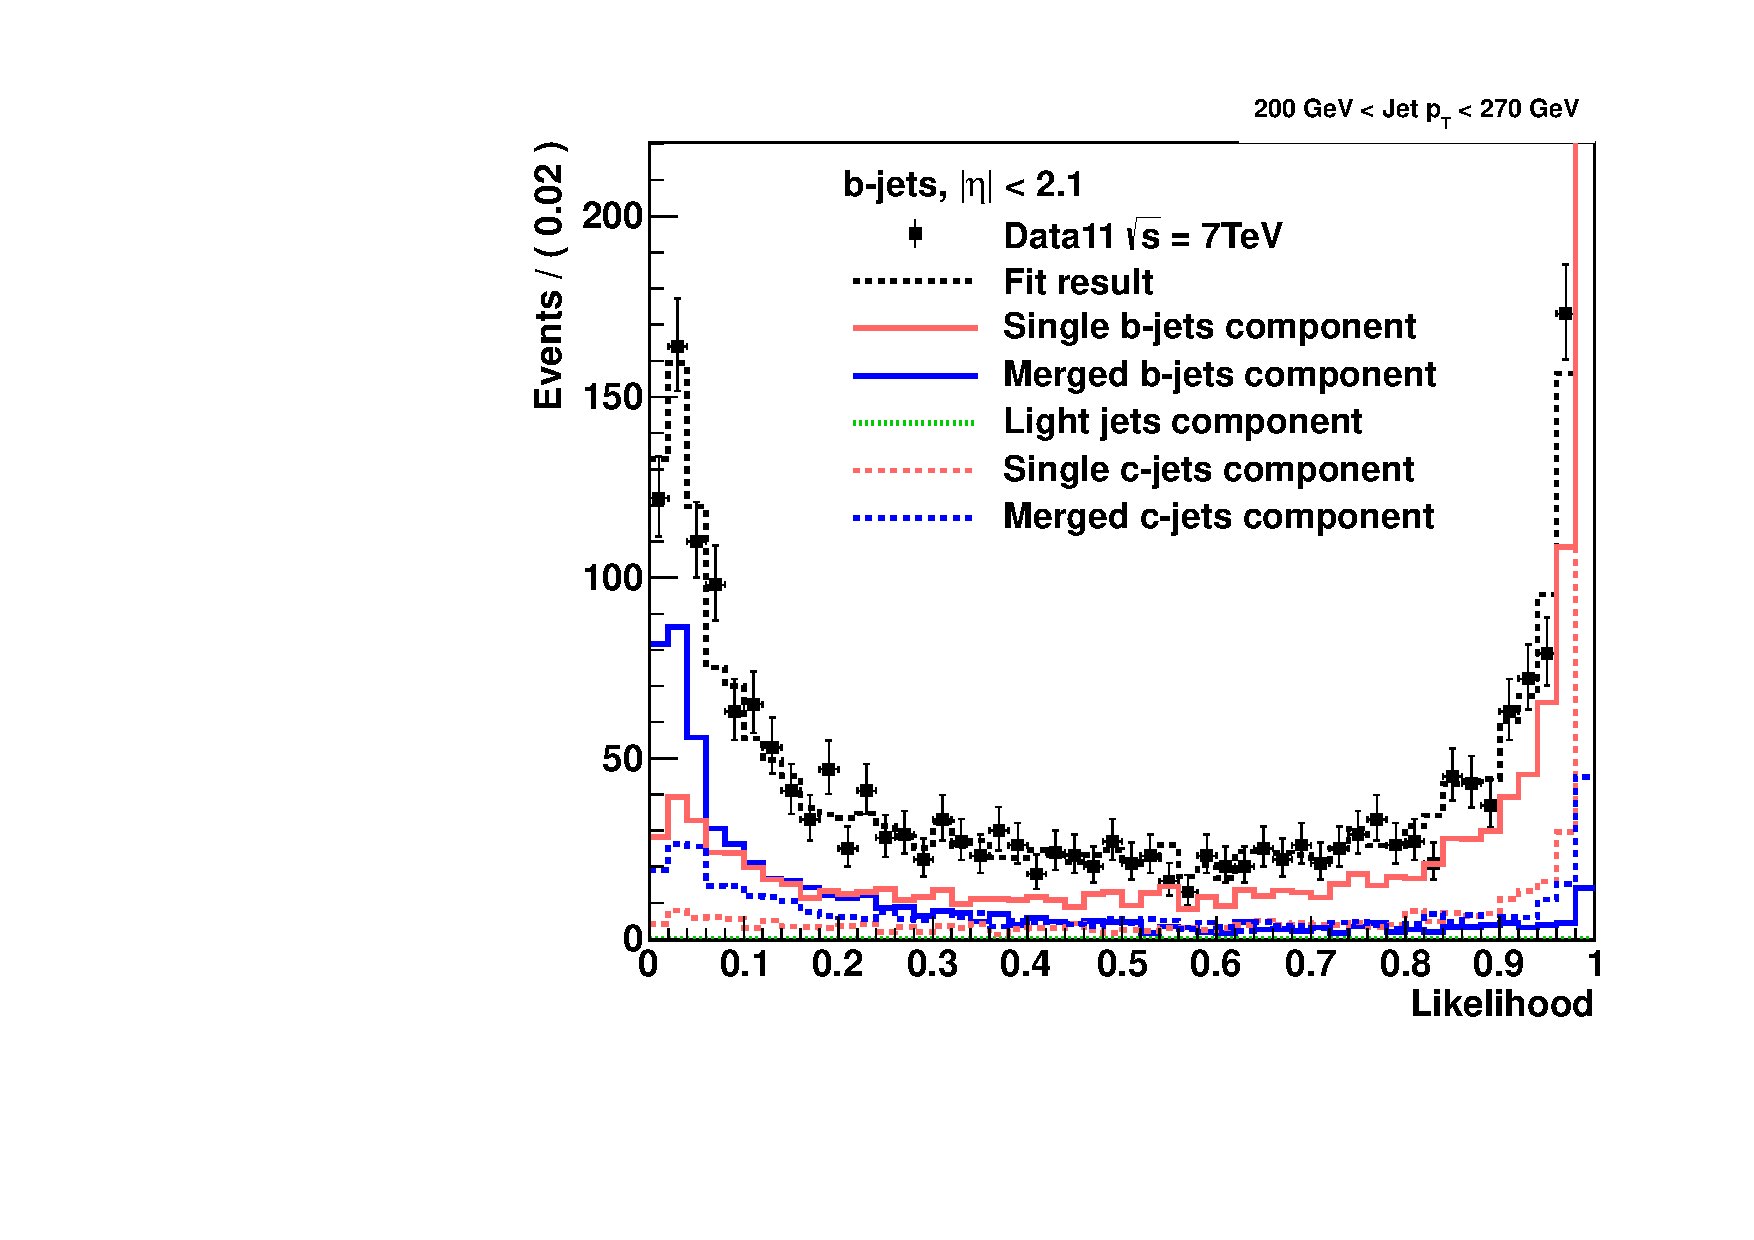
\includegraphics[width=0.7\textwidth]{FIGS/Fits/LikelihoodFit_3param_ETAFull_ZOOM_Bin5.pdf}
\caption{Example result of a template fit to the likelihood distribution in data. The fit is shown for jets with $\pt$ between  200~GeV and 270~GeV, in full scale (top) and zooming the vertical scale, to better display the flavour content of the data (bottom). Uncertainties shown are statistical only.}
\label{fig:fittemplates2}
\end{figure}

The fit results are summarized in Table~\ref{tb:fitfractions} for all $\pt$ bins, together with the theoretical prediction from a {\sc Pythia} MC simulation of QCD $b$-jet production (Section~\ref{sec:MCtools}). The errors shown are statistical, and they arise from the finite statistics of the data and template samples. The level of agreement is quantified in the Table by the pulls, which correspond to the difference between data and theory normalized to the total uncertainty (pull = (data-theory)/$\sqrt{\text{stat}^2+\text{syst}^2}$, where the systematic errors are to be discussed in Section~\ref{sec:FractionSystematics}). 

The measured composition of $b$-jets is observed to be in very good agreement with the prediction from the simulation. The single $b$-jet fraction decreases as expected with $\pt$, from 63\% to 42\%, while the merged $b$-jet fraction increases, from 8\% to 20\%. The fraction of light jets is the smallest and, except at the higher $\pt$ bins, consistent with zero. The larger fraction of light jets at high $\pt$ is expected from the simulation and is due to the increasing difficulty to efficiently tag $b$-jets in the boosted regime where the tracks associated to a jet tend to be collimated within a narrow angle.


%\emph{The sensitivity of the fit result to fixing the relative flavour fractions  $c/b$ and $c\bar{c}/b\bar{b}$, for each $\pt$ bin, to the value extracted from the simulation was investigated by carrying out separate fits with a model with three free parameters only. This was motivated by the fact that templates for single $c$- (merged $c$-)  and single $b$-jets (merged $b$-jets) look very similar leading to inestabilities in the fitted $b$- and $c$-flavour fractions, caused by the high correlations between these components.  Table~\ref{tb:correlations} shows an example covariance matrix.  Parameters $p_s$ and $p_{sc}$ and, $p_m$ and $p_{mc}$ present the highest correlation coefficients ($\sim -0.6$, and $\sim -0.8$, respectively).The fractions in the {\sc Pythia} simulation  as a function of the jet $\pt$ are displayed in Fig.~\ref{fig:truefractions} for reference.}
%\begin{table}[!hbt] %[h]
%\renewcommand{\arraystretch}{1.2}
%\centering
%\begin{tabular}{ | c | ccccc |}
%\hline
%  Parameter & $p_{mc}$  & $p_s$  & $p_m$  & $p_{sc}$  &  $p_l$ \\ \hline
%  $p_{mc}$   & 1.000 &-0.464 &-0.813&  0.257 &-0.206 \\ 
%  $p_s$     & -0.464 & 1.000 & 0.325& -0.642 &-0.323 \\
%  $p_m$     &-0.813 & 0.325 & 1.000& -0.007& -0.117 \\ 
%  $p_{sc}$   &0.257 &-0.642 &-0.007 & 1.000 &-0.300 \\
%  $p_l$      & -0.206& -0.323 &-0.117 &-0.300 & 1.000 \\ \hline
%\end{tabular}
%\caption{Correlation coefficients among the parameters adjusted in the unbinned maximum likelihood template fit to data.}
%\label{tb:correlations}
%\end{table}

%\emph{The results of template fits to the likelihood distribution in data, using the three-parameter model, are summarized in table~\ref{tb:fitfractions}. Examples of this set of fits are displayed in Figures~\ref{fig:fittemplates1} and~\ref{fig:fittemplates2}. The measured fraction of merged $b$-jets increases with the calorimeter jet $\pt$,}
%
%\begin{itemize}
%\item
%$\pt>40$ GeV: above $\sim$3\% merged $b$-jets
%\item
%$\pt>80$ GeV: above $\sim$10\% merged $b$-jets
%\item
%$\pt>200$ GeV: above $\sim$20\% merged $b$-jets
% %over 95\% rejection at 50\% eff.
%\end{itemize}
%
%\emph{The fraction of single $b$-jets changes accordingly, ranging from 60\% for low transverse momentum jets, to  40\% single $b$-jets in the highest $\pt$ bin.  The fractions of single and merged $c$-jets are fixed to their $b$-counterparts and present the same tendency (not shown in table~\ref{tb:fitfractions} for brevity) . The $p_l$ parameter representing the fraction of light jets in the data sample exhibits the largest statistical fluctuations...}
%\emph{being in most cases consistent with 0\%.}





%\begin{table}[!hbt] %[h]
%\renewcommand{\arraystretch}{1.2}
%\centering
%\begin{tabular}{ | c || c | c | c || c | c | c || c | c | c ||}
%  \hline
%  Jet $\pt$ & \multicolumn{3}{c||}{single $b$-jet} & \multicolumn{3}{c||}{merged $b$-jet} & \multicolumn{3}{c||}{~light jet~}\\ \cline{2-10}
%    (GeV ) & $p_s$ & pred.& pull & $p_m$ & pred.& pull & $p_l$ & pred.& pull \\ \hline
%   40 - 60 &  62$\pm$3 & 56 & ~1.57 &  ~~3$\pm$1   & ~3 & ~0.05 &  ~4$\pm$4  & 12 & -1.75\\ 
%   60 - 80 &  62$\pm$1 & 60 & ~1.03 &  5.2$\pm$0.4 & ~5 & -0.01 &  ~2$\pm$2  & ~5 & -1.13\\ 
%   80 - 110&  57$\pm$1 & 58 & -0.62 &  8.5$\pm$0.4 & ~7 & ~0.70 &  ~3$\pm$2  & ~5 & -0.39\\ 
%  110 - 150&  55$\pm$2 & 56 & -0.27 &  ~13$\pm$1   & 10 & ~1.13 &  ~1$\pm$4  & ~5 & -0.94\\ 
%  150 - 200&  53$\pm$3 & 52 & ~0.18 &  ~15$\pm$1   & 12 & ~1.15 &  ~0$\pm$4  & ~6 & -1.30\\ 
%  200 - 270&  53$\pm$5 & 49 & ~0.84 &  ~17$\pm$1   & 16 & ~0.53 &  -1$\pm$7  & ~8 & -1.15\\ 
%  270 - 360&  48$\pm$3 & 44 & ~1.03 &  ~19$\pm$1   & 18 & ~0.40 &  ~4$\pm$4  & 11 & -1.39\\
%  360 - 480&  39$\pm$5 & 36 & ~0.41 &  ~21$\pm$1   & 21 & ~0.07 &  15$\pm$6  & 19 & -0.49\\ \hline
%\end{tabular}
%\caption{Measured proportions (in percentage) of single, merged and light $b$-tagged jets in experimental data from 2011 run.}
%\label{tb:fitfractions}
%\end{table}

\begin{sidewaystable}[!hbtp] %[h]
\renewcommand{\arraystretch}{1.2}
%\centering
\begin{tabular}{ | c || c | c | c || c | c | c || c | c | c || c | c | c || c | c | c ||}
  \hline
  Jet $\pt$ & \multicolumn{3}{c||}{single $b$-jet} & \multicolumn{3}{c||}{merged $b$-jet} 
            & \multicolumn{3}{c||}{~light jet~}    & \multicolumn{3}{c||}{single $c$-jet} 
            & \multicolumn{3}{c||}{merged $c$-jet}
            \\ \cline{2-16}
    (GeV)  &\,data\,&\!\!theory\!\!&\:pull\:&\,data\,&\!\!theory\!\!&\:pull\:&\,data\,&\!\!theory\!\!&\:pull\:&\,data\,&\!\!theory\!\!&\:pull\:&\,data\,&\!\!theory\!\!& pull\\ \hline
   40 - 60 & 63$\pm$4~& 56 & ~1.49 &  8$\pm$1 & 3   & ~2.10 & ~4$\pm$4 &  12 &  -1.65 & 31$\pm$2 & 24 & ~2.51 & -7$\pm$3 &   5 & -2.82\\ 
   60 - 80 & 59$\pm$2~& 60 & -0.13 &  5$\pm$1 & 5   & ~0.02 & ~2$\pm$2 &  ~5 &  -1.15 & 26$\pm$1 & 23 & ~1.26 & ~8$\pm$2 &  ~7 & ~0.30\\ 
   80 - 110& 56$\pm$3~& 58 & -0.77 & 12$\pm$1 & 7   & ~1.80 & ~3$\pm$2 &  ~5 &  -0.35 & 24$\pm$2 & 22 & ~0.66 & ~5$\pm$2 &  ~8 & -0.88\\ 
  110 - 150& 49$\pm$5~& 56 & -1.23 & 12$\pm$2 & 10  & ~0.69 & -1$\pm$4 &  ~5 &  -1.22 & 25$\pm$4 & 21 & ~1.01 & ~5$\pm$3 &  ~9 & ~1.35\\ 
  150 - 200& 47$\pm$5~& 52 & -2.64 & 13$\pm$2 & 12  & ~0.25 & -1$\pm$4 &  ~6 &  -1.58 & 31$\pm$4 & 19 & ~2.74 & 10$\pm$3 &  10 & ~2.49\\ 
  200 - 270&\!\!51$\pm$12\!\!& 49 & ~0.21 & 19$\pm$3 & 16  & ~0.77 & ~1$\pm$7 &  ~8 &  -0.89 & 19$\pm$8 & 16 & ~0.32 & 10$\pm$5 &  12 & -0.22\\ 
  270 - 360& 51$\pm$4~& 44 & ~1.34 & 22$\pm$1 & 18  & ~1.45 & ~7$\pm$4 &  11 &  -0.95 & 13$\pm$3 & 13 & -0.14 & ~8$\pm$2 &  13 & -1.64\\
  360 - 480& 42$\pm$7~& 36 & ~0.73 & 19$\pm$1 & 21  & -0.64 & 13$\pm$6 &  19 &  -0.82 & ~9$\pm$5 & 11 & -0.33 & 17$\pm$2 &  14 & ~1.02\\ \hline
\end{tabular}
\caption{Measured proportions (in percentage) of the composition of $b$-jets in QCD production, compared to the theoretical prediction from a MC {\sc Phythia} simulation. Errors shown are only statistical. The pull corresponds to (data-theory)/$\sqrt{\text{stat}^2+\text{syst}^2}$}
\label{tb:fitfractions}
\end{sidewaystable}
                   



%------------------------------------------------------------------------
\section{Systematic uncertainties}\label{sec:FractionSystematics}
%------------------------------------------------------------------------

The systematic uncertainties affecting the compostion measurement are mainly those that change the shape of the likelihood templates. The following sources were evaluated:

\begin{itemize}\addtolength{\itemsep}{-0.4\baselineskip}
\item
track reconstruction efficiency;
\item
jet transverse momentum resolution 
\item
jet energy scale.
%\item
%uncertainty in the heavy flavor fraction
\end{itemize}


In order to calculate the contribution from the uncertainty in the track reconstruction efficiency a random fraction of the tracks were discarded following the procedure described in Section~\ref{sec:gbbSystematics}. New likelihood templates were produced from the modified events and the fits redone with them. 

The systematic uncertainty originating from the jet  $\pt$ resolution is obtained by over-smearing the calorimeter jet $\pt$ in the simulation. The likelihood templates were rederived from this smeared sample, and the likelihood distribution in data fit using these altered samples. The difference between the unsmeared and the smeared scenarios is taken as the systematic error. 

The uncertainty originating from the jet energy scale is obtained by scaling the $\pt$ of each jet in the simulation up and down by one standard deviation, according to the uncertainty of the jet energy scale (see Section~\ref{sec:gbbSystematics}), and redoing the likelihood fits on data with the modified  %$b$, $c$, $b\bar{b}$, $c\bar{c}$ and light 
templates.

%The impact of the uncertainty in the knowledge of the relative flavour fractions $c/b$ and $c\bar{c}/b\bar{b}$ fractions in the simulation was evaluated by separately changing these ratios by 20\%. The variation in the ratio $c\bar{c}/b\bar{b}$ only produced a marginal effect on the fit results. The total number of merged $c$ plus merged $b$ did not change showing that, although a separate value for the $b\bar{b}$- and $c\bar{c}$-flavoured components can be obtained, we are,  in reality, measuring the fraction of merged $b\bar{b}+c\bar{c}$ together. The same result is observed if changing the single $c/b$ ratio.

The resulting systematic uncertainties are summarized in Table~\ref{tb:systematicsfits}. The largest contributions arise from the jet energy scale and jet transverse momentum resolution.
\begin{table}[!hbt] %[h]
\renewcommand{\arraystretch}{1.2}
\centering
\begin{tabular}{ | c | c |}
\hline
  ~~~~~~~Systematic source~~~~~~~ &~~Uncertainty~~\\ \hline
  track reconstruction efficiency  &    negligible        \\ 
  jet $\pt$ resolution  &    1\%        \\  
  jet energy scale  &    2\%        \\ 
%  heavy flavour fraction  &    negligible        \\ 
\hline 
\end{tabular}
\caption{Contributions to the systematic uncertainties affecting the template fitting to experimental data.}
\label{tb:systematicsfits}
\end{table}


%------------------------------------------------------------------------
\section{Enriched single and merged {\em b}-jet samples}\label{sec:Enriched}
%------------------------------------------------------------------------

The inclusive QCD data sample is $\sim$50\% pure in single $b$-jets, according to the measurements described in Section~\ref{sec:FitsResults}. It is interesting to envisage the use of semi-inclusive samples, defined with adequate selection cuts to have a higher composition in single or in merged $b$-jets. On the one hand, this can be used to test the theoretical picture of QCD $b$-jet production. On the other, it would help validate the universality of the Monte Carlo templates used for fitting. 
%To this end we consider the Monte Carlo dijet sample to determine the purity than can be achieved by simple kinematic and $b$-tagging cuts, leaving reasonable statistics.

As discussed in Section~\ref{sec:bjet-production}, single $b$-jets are produced via the Flavour Creation (FCR) and Flavour Excitation (FEX) processes.  In the former two heavy quarks are produced in the hard scatter, yielding two hard $b$-quarks in the final state. The latter can be depicted as an initial state gluon splitting into a $b\bar{b}$ pair, where one of the $b$-quarks subsequently scatters off a parton in the opposite proton, yielding one hard $b$-quark and one forward $b$-quark in the final state.
Merged $b$-jets are produced mostly by Gluon Splitting (GSP). In this process no heavy quarks participate in the hard scatter, but they are produced via the subsequent $g \rightarrow b\bar{b}$ branching with both $b$-quarks clustered in the same jet. 

In the FCR process the two $b$-quarks give rise to a back-to-back pair of single $b$-jets in the transverse plane\footnote{The presence of jets from initial and final state radiation distorts this simplified picture. This sentence should thus be understood as a first order description of the process.}. On the contrary, FEX and GSP also give rise to two back-to-back jets, but with only one of them containing heavy flavor. This picture suggests that requiring events with two $b$-tags is an efficient way to build a sample enriched in single $b$-jets.  On the other hand, requesting events with only one $b$-tag enriches the FEX and GSP contributions, giving rise to a light jet plus a single or merged $b$-jet, respectively.
%can be produced either in the FEX process, with only one central $b$-quark in the final state, or via GSP, where $b\bar{b}$ pairs produced at small angles can be reconstructed as a single $b$-jet. 
These two scenarios are more difficult to disentangle. %and will require further selection cuts to be applied.

\subsubsection{Purified sample in single {\em b}-jets}

A sample enriched in single $b$-jets is achieved by restricting the data to events with exactly two $b$-tags,
%To help purify the sample in single $b$-jets we can then use the $b$-tagging information. Jets in data events with exactly two $b$-tags, 
selected with the MV1 tagging algorithm at its 60\% working point and satisfying the event and jet selection described in Section~\ref{sec:EventSelection}.
% compose the purified data set.  
In order to increase the statistics no requirement on the $\pt$ of the second $b$-tagged jet is imposed. 
This sample is expected to be very pure, albeit with some contamination from FEX and GSP due to mistags, where the accompanying jet is incorrectly tagged as a $b$.

\begin{table}[!hbt] %[h]
\renewcommand{\arraystretch}{1.2}
\centering
\begin{tabular}{ | c || c | c | c || c | c | c ||}
  \hline
  Jet $\pt$ & \multicolumn{3}{c||}{single $b$-jets}& \multicolumn{3}{c||}{merged $b$-jets}\\ \cline{2-7}
    (GeV) & ~~data~~ & ~theory~ & ~~~pull~~~& ~~data~~ & ~theory~ & ~~~pull~~~\\ \hline
   40 - 60 &  99$\pm$11 & 84   & ~1.37&  -1$\pm$1& 1 &-0.74 \\  
   60 - 80 &  82$\pm$5  &  87  & -1.01&  -3$\pm$1& 1 &-1.60 \\ 
   80 - 110&  84$\pm$5  &  88 &  -0.72&  ~2$\pm$1& 1 &~0.37 \\ 
  110 - 150&  86$\pm$8  &  85 &  ~0.02&  ~4$\pm$2& 3 &~0.41 \\ 
  150 - 200&  89$\pm$9  &  83 &  ~0.67&  ~4$\pm$2& 3 &~0.20 \\ 
  200 - 270&  95$\pm$5  &  80 &  ~1.00&  ~7$\pm$2& 5 &~0.61 \\ 
  270 - 360&  67$\pm$11  &  81 & -1.25&  12$\pm$2& 6 &~2.21 \\ 
  360 - 480&  73$\pm$16  &  73 & -0.01&  10$\pm$1& 8 &~0.98 \\ \hline
\end{tabular}
\caption{Percentage of single  and merged $b$-jets in a QCD sample enriched in single $b$-jets by requiring events with two $b$-tags. See details in the text.} %in experimental data from 2011 run, enriched in single $b$-jets.}
\label{tb:fitfractions2btagS}
\end{table}
%Once the enriched sample is obtained, new likelihood fits are performed for all $\pt$ bins, utilizing the same MC templates as for the inclusive data sample.  
The likelihood fits are performed on the purified sample, utilizing the same MC templates as for the inclusive case.
The measured fractions of single and merged $b$-jets, together with their statistical errors and {\sc Pythia} MC predictions for each $\pt$ bin are displayed in Table~\ref{tb:fitfractions2btagS}. The agreement between theory and experiment is excellent. The fraction of single (merged) $b$-jets substantially increases (decreases) as expected, confirming the intuitive picture discussed in Section~\ref{sec:bjet-production} in terms of Feynman diagrams.


An example of the enriched template fits is shown in Figure~\ref{fig:fitenriched2btag1}, comparing for the same $\pt$ bin the inclusive and the semi-inclusive single-$b$ enriched cases.  % and Figures~\ref{fig:fitenriched2btag2}. 
The template description agrees very well within statistics with the data. In fact, even by ocular inspection it can be ascertained that the merged-$b$ fraction decreases, given the evident reduction in the peak at low LL. 
% and the result is in good agreement with the predictions made by {\sc Pythia} on a sample with the same level of enrichment.  
\begin{figure}[tp]
\centering
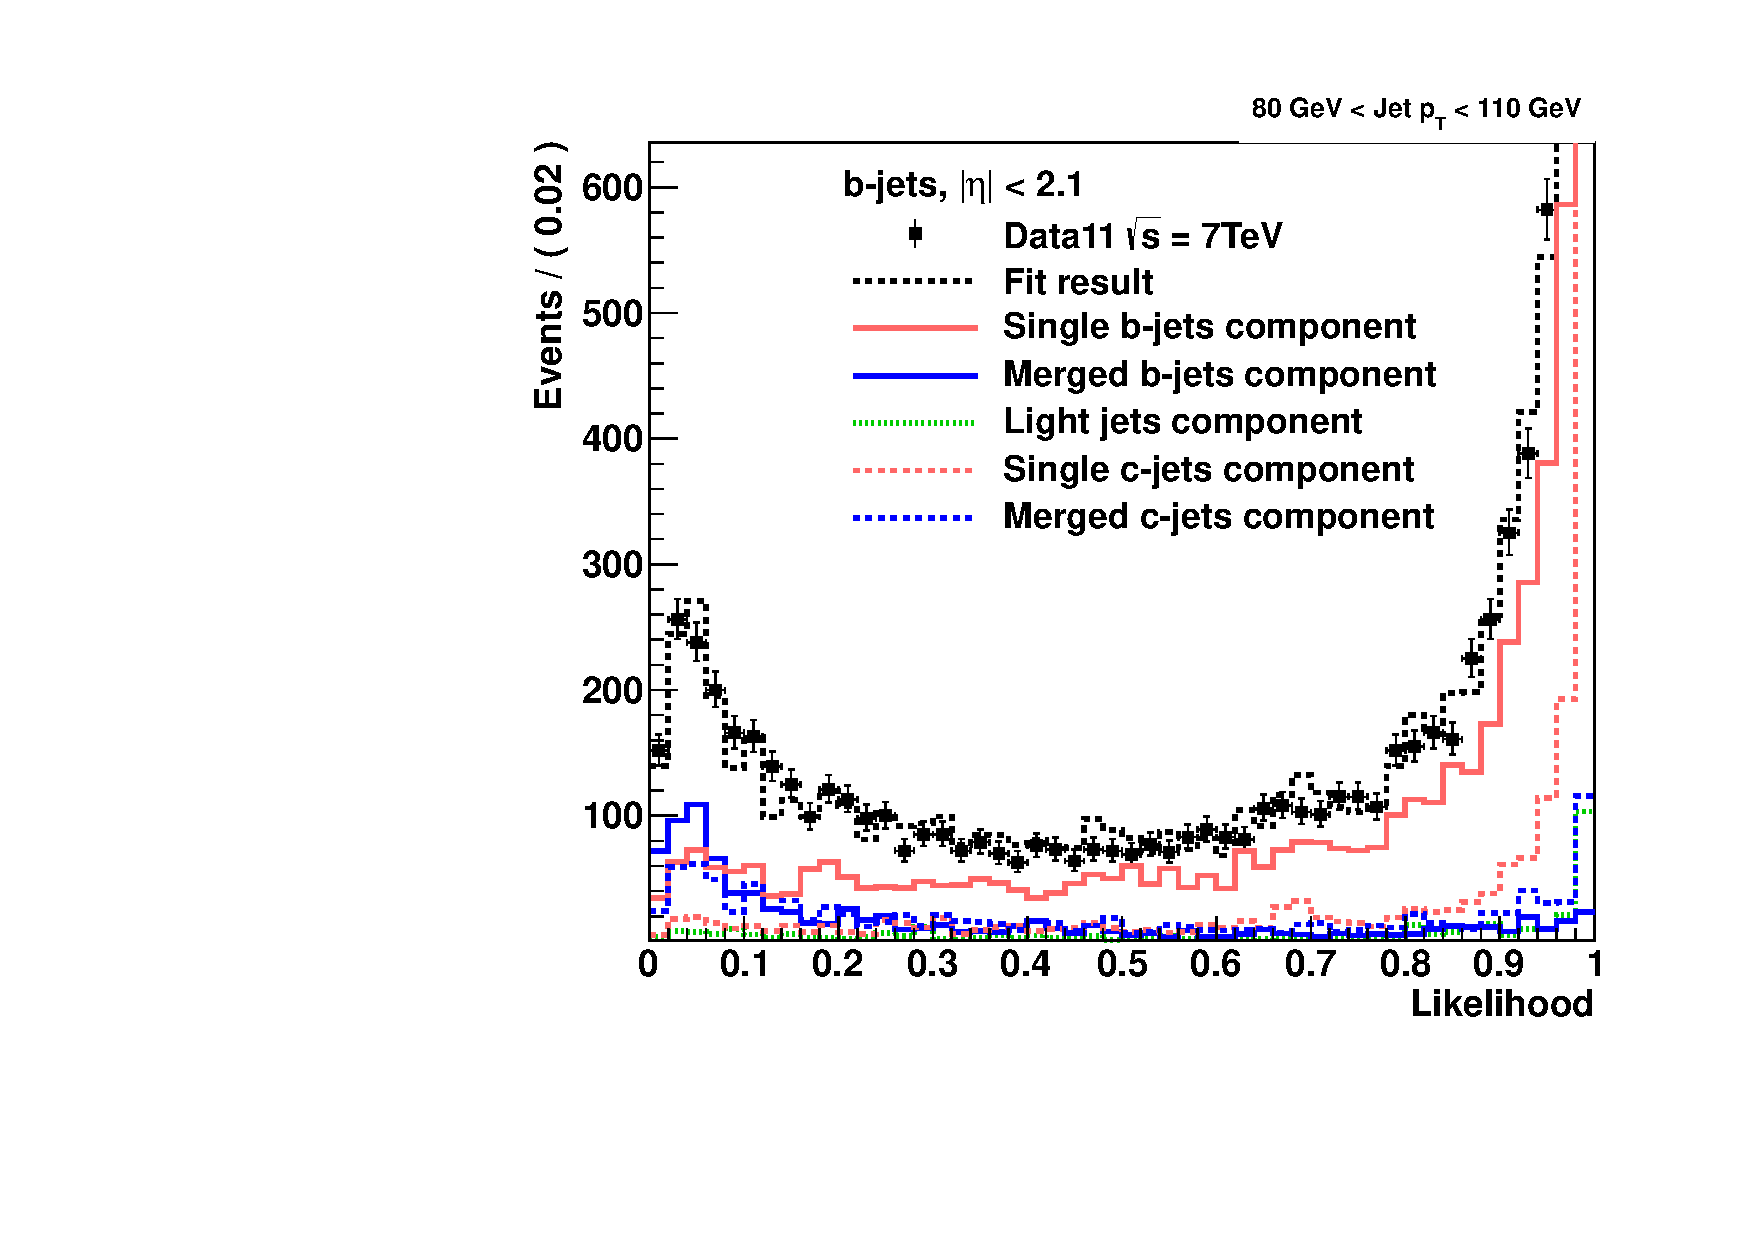
\includegraphics[width=0.7\textwidth]{FIGS/Fits/LikelihoodFit_3param_ETAFull_ZOOM_Bin2.pdf}
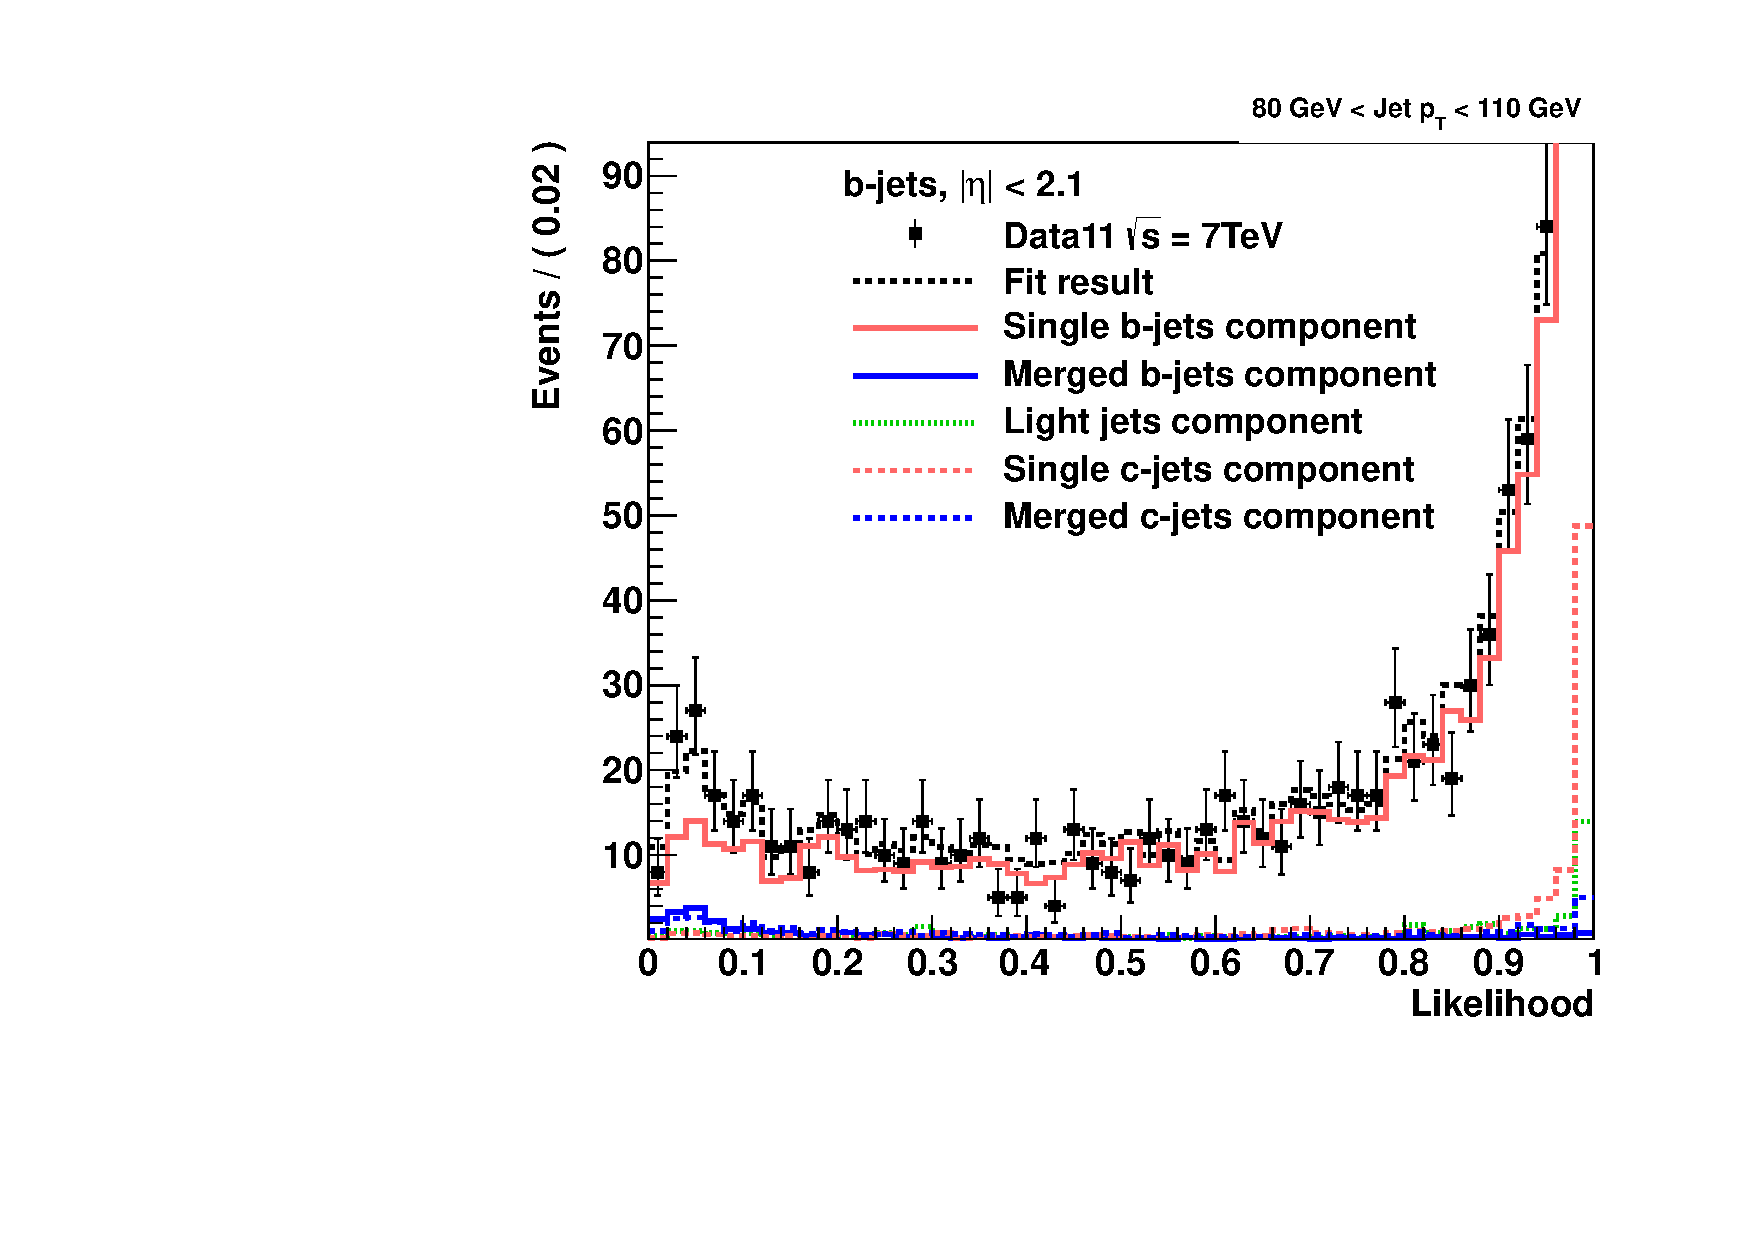
\includegraphics[width=0.7\textwidth]{FIGS/Fits/LikelihoodFit_3param_ETAFull_DataEnriched2btagZOOMtest_Bin2.pdf}
\caption{Example result of a template fit to the likelihood distribution in the semi-inclusive single-$b$ enriched sample for jets with $\pt$ between  80~GeV and 110~GeV (bottom).  The result for the same  $\pt$ bin in the inclusive sample is also shown for comparison (top).  The vertical scale was enlarged in the two plots to better appreciate all contributions. Uncertainties shown are statistical only.}
\label{fig:fitenriched2btag1}
\end{figure}

\subsubsection{Purified sample in merged {\em b}-jets}

Events with only one $b$-tagged jet were selected for the purification of the data sample in double $b$-hadron jets.  In order to reinforce this selection, a tight anti-$b$-tagging requirement on any non-tagged jet in the event was implemented.  The anti-$b$-tagging was performed by imposing, simultaneously, strict cuts on the $b$-tag weights of the three supported taggers available within ATLAS:
%
\begin{itemize}
\item
MV1:  $w < 0.07$  
\item
JetFitter:  $w < -2$
\item
IP3D+SV1:  $w < -2$
\end{itemize}
%
These weight values correspond to a MV1 tagging efficiency of more than 85\%, and an efficiency for $b$-tagging of more than 80\% for the JetFitter and IP3D+SV1 algorithms. These high efficiencies are chosen because we want to safely veto on the second jet and do not mind if the price is a high level of fake vetos. %a high level of contamination.

The idea behind the anti-b-tagging requirement is to eliminate FCR events for which one of the produced $b$-quark jets failed to be tagged. However, although a certain level of purification was expected, very little enrichment was achieved with this kind of selection. %The results from these fits (the fractions of merged $b$-jets in the enriched sample) are presented in  table~\ref{tb:fitfractions2btagM}.

The results are summarized in Table~\ref{tb:fitfractions2btagM}, which shows the measured fractions of single and merged $b$-jets, together with their statistical errors and {\sc Pythia} MC predictions for each $\pt$ bin. Although there is good agreement between data and experiment, it is clear that a much lower level of purification has been achieved than for the previous case of single $b$-tagged jets. This was expected, given that the selection cuts enhance the composition not only of the GSP, but also the FEX component. 
Some further studies were performed but with only relative success. In particular the $b$-tagged jet was requested to be back-to-back to the highest (or second highest) $\pt$ jet in the event.  Back-to-back jets were defined as those satisfying:  $\Delta R>2.8$ and  $\pt^\text{tagged}/\pt^\text{leading} > 0.7$  (if the $b$-tagged jets is the leading one, the cut is replaced by $\pt^\text{subleading}/\pt^\text{tagged} > 0.7$). No improvement was found either by restrintig to the case where the $b$-jet is the leading or the sub-leading one.

%\emph{Further studies were performed requiring the $b$-tagged jet in the event to be back-to-back to the highest (second highest) $\pt$ jet in the event.  Back-to-back jets were defined as those satisfying:  $\Delta R>2.8$ and  $\pt^{tagged}/\pt^{lead} > 0.7$  (in the case the $b$-tagged jets is the leading jet of the event, this cut is $\pt^{second}/\pt^{tagged} > 0.7$). Actually, most of the $b$-tagged jets in one-$b$-tagged events fall in this category. Three different topologies are expected to be left after the selection described above: FCR back-to-back single $b$-jets not tagged,  FEX single $b$-jets back-to-back with light jets, and GSP merged $b$-jets, also back-to-back with light. In oder to enrich the sample in merged $b$-jets one would like to reduce the rate of the first two configurations.  It was found that in 90\% of these cases the  non-tagged jet is a light jet. This observation imposes a limitation on how far one can go in purifying the QCD sample since $b$-jets arising from FEX process constitute and irreducible background for selecting merged $b$-jets. Other physics samples would be required in order to obtain a reasonable enrichment.}

%\begin{figure}[tp]
%\centering
%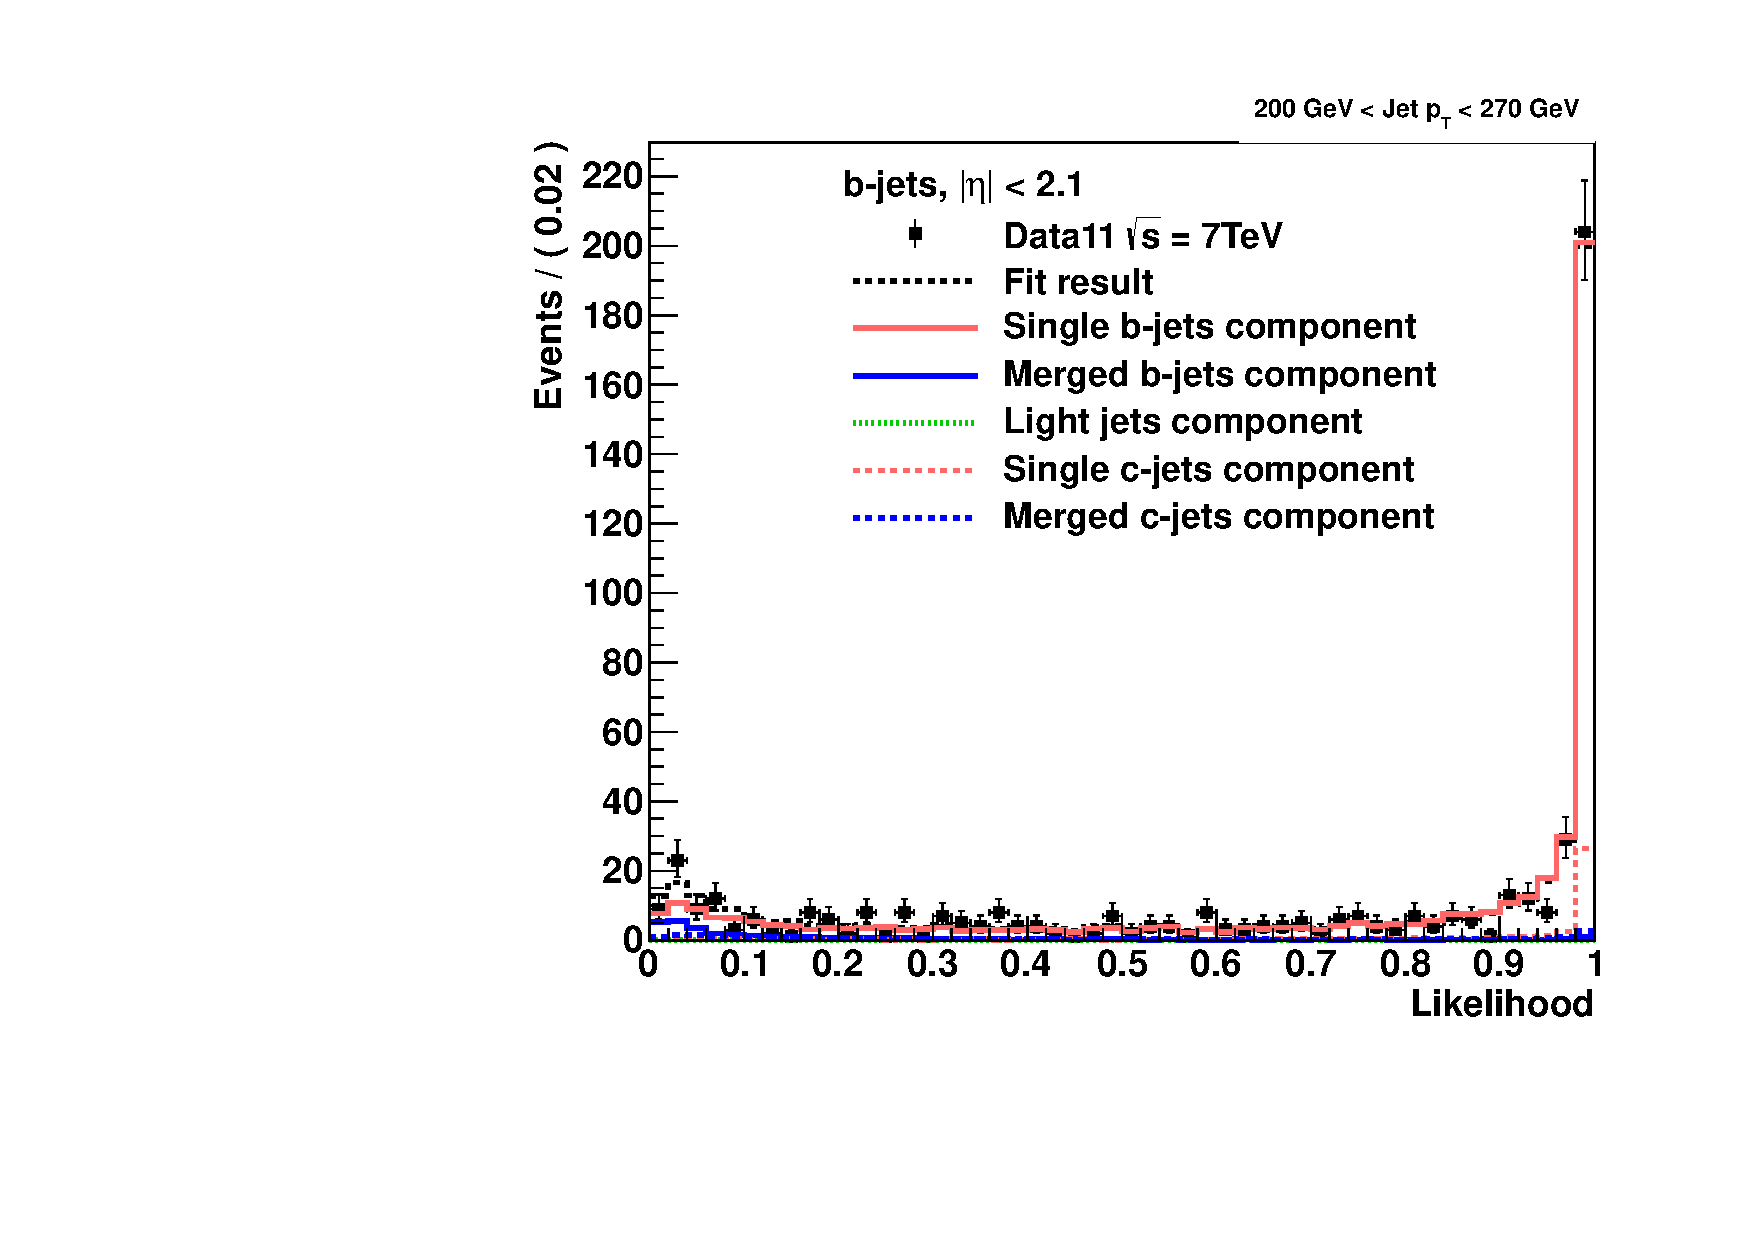
\includegraphics[width=0.7\textwidth]{FIGS/Fits/LikelihoodFit_3param_ETAFull_DataEnriched2btag_Bin5.pdf}
%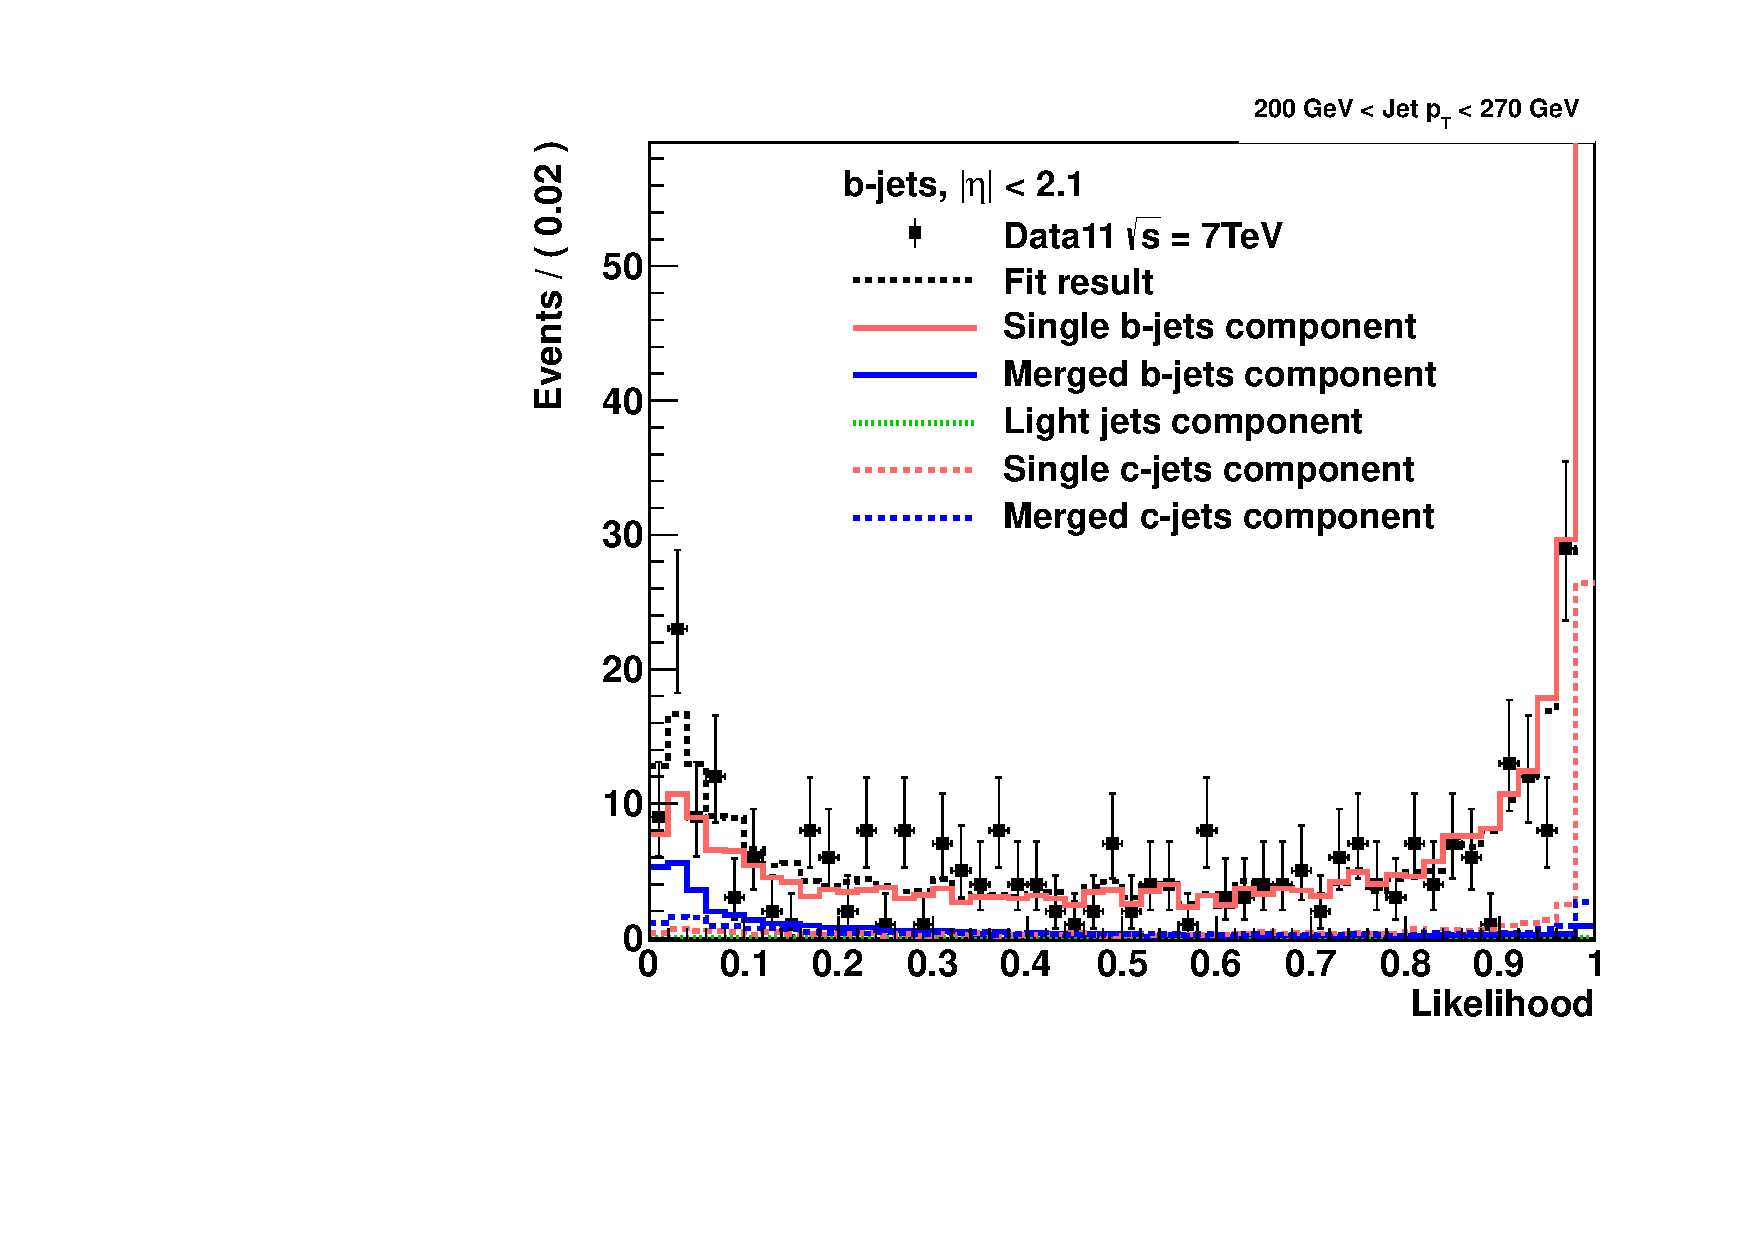
\includegraphics[width=0.7\textwidth]{FIGS/Fits/LikelihoodFit_3param_ETAFull_DataEnriched2btagZOOM_Bin5.pdf}
%\caption{Example result of a template fit to the likelihood distribution in data enriched in single $b$-jets. The fit is shown for jets with $\pt$ between  200~GeV and 270~GeV, in full scale (top) and zooming the vertical scale, to better display the flavour content of the data (bottom). Uncertainties shown are statistical only.}
%\label{fig:fitenriched2btag2}
%\end{figure}
%\begin{table}[!hbt] %[h]
%\renewcommand{\arraystretch}{1.2}
%\centering
%\begin{tabular}{ | c || c | c | c ||}
%  \hline
%  Jet $\pt$ & \multicolumn{3}{c||}{merged $b$-jet}\\ \cline{2-4}
%    (GeV ) & ~~~~fit result~~~ & ~~~~stat.err.~~~~ & pythia prediction \\ \hline
%   40 - 60 &  -1\%  &  1\%  &  1\% \\  
%   60 - 80 &  -3\%  &  1\%  &  1\% \\ 
%   80 - 110&  ~2\%  &  1\%  &  1\% \\ 
%  110 - 150&  ~4\%  &  2\%  &  3\% \\ 
%  150 - 200&  ~4\%  &  2\%  &  3\% \\ 
%  200 - 270&  ~7\%  &  2\%  &  5\% \\ 
%  270 - 360&  12\%  &  2\%  &  6\% \\ 
%  360 - 480&  10\%  &  1\%  &  8\% \\ \hline
%\end{tabular}
%\caption{Measured proportions of merged $b$-jets in experimental data from 2011 run, enriched in single $b$-jets.}
%\label{tb:fitfractions2btagM}
%\end{table}

\begin{table}[!hbt] %[h]
\renewcommand{\arraystretch}{1.2}
\centering
\begin{tabular}{ | c || c | c | c || c | c | c ||}
  \hline
  Jet $\pt$ & \multicolumn{3}{c||}{single $b$-jets}& \multicolumn{3}{c||}{merged $b$-jets}\\ \cline{2-7}
    (GeV) & ~~data~~ & ~theory~ & ~~~pull~~~ & ~~data~~ & ~theory~ & ~~~pull~~~\\ \hline
   40 - 60   &  58$\pm$3 &  53   &  ~1.50   &  ~4$\pm$1    &  ~~3  &  ~0.26 \\  
   60 - 80   &  58$\pm$1 &  55   &  ~1.25   &  6.1$\pm$0.5  &  5.9  &  ~0.09 \\ 
   80 - 110  &  51$\pm$1 &  52   &  -0.42   &  9.4$\pm$0.5  &  8.2  &  ~0.55 \\ 
  110 - 150  &  48$\pm$2 &  48   &  ~0.15   &  14$\pm$1    &  ~12  &  ~1.10 \\ 
  150 - 200  &  45$\pm$3 &  44   &  ~0.38   &  17$\pm$1    &  ~15  &  ~0.86 \\ 
  200 - 270  &  44$\pm$5 &  40   &  ~0.74   &  20$\pm$1    &  ~19  &  ~0.24 \\ 
  270 - 360  &  41$\pm$3 &  34   &  ~1.80   &  21$\pm$1    &  ~22  &  -0.30 \\ 
  360 - 480  &  32$\pm$5 &  29   &  ~0.59   &  23$\pm$1    &  ~23  &  -0.34 \\ \hline
\end{tabular}
\caption{Proportion (in percentage) of single and merged $b$-jets in a QCD sample enriched in merged $b$-jets by requiring events with only one $b$-tag. See details in the text.}
%\caption{Measured proportions of merged $b$-jets in experimental data from 2011 run, enriched in merged $b$-jets.}
\label{tb:fitfractions2btagM}
\end{table}


